% Template for PLoS
% Version 1.0 January 2009
%
% To compile to pdf, run:
% latex plos.template
% bibtex plos.template
% latex plos.template
% latex plos.template
% dvipdf plos.template

\documentclass[10pt]{article}

% amsmath package, useful for mathematical formulas
\usepackage{amsmath}
% amssymb package, useful for mathematical symbols
\usepackage{amssymb}

% graphicx package, useful for including eps and pdf graphics
% include graphics with the command \includegraphics
\usepackage{graphicx}

% cite package, to clean up citations in the main text. Do not remove.
\usepackage{cite}

\usepackage{color} 

\usepackage{marginnote}

% Use doublespacing - comment out for single spacing
\usepackage{setspace} 
\doublespacing

% enumitem - package to compress lists
\usepackage{enumitem}

% Text layout
\topmargin 0.0cm
\oddsidemargin 0.5cm
\evensidemargin 0.5cm
\textwidth 16cm 
\textheight 21cm

% Bold the 'Figure #' in the caption and separate it with a period
% Captions will be left justified
\usepackage[labelfont=bf,labelsep=period,justification=raggedright]{caption}

% Use the PLoS provided bibtex style
\bibliographystyle{./plos2009}

% Remove brackets from numbering in List of References
\makeatletter
\renewcommand{\@biblabel}[1]{\quad#1.}
\makeatother
%\renewcommand{\paragraph}[1]{{#1}}

% Leave date blank
\date{}

\pagestyle{myheadings}
%% ** EDIT HERE **


%% ** EDIT HERE **
%% PLEASE INCLUDE ALL MACROS BELOW

%% END MACROS SECTION

\begin{document}

% Title must be 150 characters or less
\begin{flushleft}
{\Large
\textbf{A Federated Design for a Neurobiological Simulation Engine: The CBI federated software architecture.}
}
% Insert Author names, affiliations and corresponding author email.
\\
Hugo Cornelis$^{1,\ast}$, 
Allan D. Coop$^{2}$,
James M. Bower$^{3}$.
\\
\bf{1} Cornelis H. Research Imaging Institute, University of Texas Health Science Center at San Antonio, San Antonio, TX, United States
\\
\bf{2} Coop A. D. Deptartment of Epidemiology and Biostatistics, University of Texas Health Science Center at San Antonio, San Antonio, TX, United States
\\
\bf{3} Bower J. M. Research Imaging Institute, University of Texas Health Science Center at San Antonio, San Antonio, TX, United States
\\
$\ast$ E-mail: Corresponding Hugo.Cornelis@gmail.com
\end{flushleft}

% Please keep the abstract between 250 and 300 words
\section*{\LARGE Abstract}

Simulator\marginnote{
  \begin{picture}(0,0)
    \put(-10,10){\line(0,-1){0}}
  \end{picture}
} interoperability and extensibility has become a growing requirement in computational biology. To address this, we have developed a federated software architecture. It is
federated by its union of independent disparate systems under a single
cohesive view, provides interoperability through its capability to
communicate, execute programs, or transfer data among different
independent applications, and supports extensibility by enabling simulator expansion or enhancement without the need for major changes to system infrastructure.

Historically, simulator interoperability has relied on development of
declarative markup languages such as the neuron modeling language
NeuroML, while simulator extension typically occurred through
modification of existing functionality.  The software architecture we
describe here allows for both these approaches. However, it is
designed to support alternative paradigms of interoperability and
extensibility through the provision of logical relationships and defined application
programming interfaces.  They allow any appropriately configured
component or software application to be incorporated into a simulator.

The architecture defines independent functional modules that run
stand-alone. They are arranged in logical layers that naturally
correspond to the occurrence of high-level data (biological concepts)
versus low-level data (numerical values) and distinguish data from
control functions.

The modular nature of the architecture and its independence from a
given technology facilitates communication about similar concepts and
functions for both users and developers.  It provides several
advantages for multiple independent contributions to software
development.  Importantly, these include: (1) Reduction in complexity
of individual simulator components when compared to the complexity of
a complete simulator, (2) Documentation of individual components in
terms of their inputs and outputs, (3) Easy removal or replacement of
unnecessary or obsoleted components, (4) Stand-alone testing of
components, and (5) Clear delineation of the development scope of new
components.

% Here, we introduce and describe the Computational Biology Initiative federated software architecture.

%\marginpar{{\bf Hugo:} Currently 282 words, must be $\leq$ 300.}

%Software architectures can be described in different ways.  This paper
%describes the CBI simulator software architecture by putting
%stand-alone software components into a logically layered diagram.  The
%layers in the software architecture naturally correspond to the
%occurence of high-level data (e.g. biological concepts) versus
%low-level data (e.g.  numerical values).  This diagram can be used by
%users as well as developers to communicate about the global concepts
%and functions present in the software, independent of the used
%technology.
%
%Each software component is self-contained, in the sense that it can be
%run stand-alone. This has important advantages for
%facilitating contributions to software development from many people:
%
%\begin{itemize}
%\item The complexity of a single component is reduced compared to the
%  complexity of a complete software system.
%\item A component can be documented as an isolated entity, in terms of
%  inputs and outputs.  This facilitates the communication between
%  developers.
%\item When a component is considered not necessary or obsoleted, it
%  can be replaced, or removed from the architecture.
%\item From a developer perspective, a component can be tested
%  stand-alone.
%\item Most importantly, for new developments, the architecture clearly
%  delineates the scope of the development.  From the early start, new
%  components can be designed to fill only one component of the
%  architecture.
%\end{itemize}
%
%These properties facilitate the building and maintenance of a
%developer community, and the integration of new components.
%
%The CBI simulator software architecture is the result of a functional
%analysis of user requirements.  It indirectly represents the user
%needs, independent of concerns such as the technology used or the
%technical requirements (so also independent of the fact if it is
%technically possible to implement this architecture).  Since users can hook in
%extensions at a layer that is clearly defined, this analysis also
%provides an infrastructure for extensibility.
%
%discuss operations modelers perform on a model, taken from thesis
%
%say that a model evolves over time, discuss shortly the purkinje cell
%model, macro evolution.  Discuss operations in context of a data model
%?
%
%Relate the data model to an XML data model, more specifically neuroml data model.
%
%discuss the ndf data model, include an example.
%
%Link with
%http://en.wikipedia.org/wiki/High\_Level\_Architecture \\
%http://en.wikipedia.org/wiki/Levels\_of\_conceptual\_interoperability \\
%http://en.wikipedia.org/wiki/Data\_integration \\
%http://en.wikipedia.org/wiki/Abstraction\_layer \\
%
%accessibility for neuronal model parameters:
%
%e.g. conductance vs scaled conductance.
%
%conductance scaling contains a set of logic rules:
%1. for a simple compartment
%2. for a compartment with spines
%3. for specific membrane resistance.

\section*{\LARGE Introduction}

The application of mathematical methods to modeling and quantification in neurophysiology can be traced to the Lapicque model of a neuron introduced over a century ago \cite{L:1907fk}, the empirical description of action potential generation and propagation \cite{hodgkin52:_quantitative_description}, the application of cable theory to the modeling of dendritic electrophysiology \cite{Rall:1957uq}, and the recognition that different levels of analysis could be employed to understand brain function \cite{Marr:1982fk}. Although, a hand cranked calculator was employed to verify the original integration of the action potential, it was not until mathematical approaches based on cable theory were developed to model dendritic properties and function in the late 1950s, that digital computers became a necessary tool for modeling studies  \cite{rall59:_branc}. It took a further quarter century for the interdisciplinary field that links neuroscience, cognitive science, electrical engineering, computer science, physics, and mathematics to be named and thus give birth to computational neuroscience \cite{Schwartz:1990kx}.
%Since that time, a continued and rapid development of computer hardware and software has led to a plethora of systems for the description, simulation, and analysis of computational models from the sub-cellular (e.g. MCell--Stiles \& Bartoll, 2001; Roth et al., 2000) to large networks of biophysically realistic model neurons (e.g. Brunel \& Wang, 2001, Traub et al., 2005).

% Lapicque L (1907) Recherches quantitative sur l'excitabilitie electrique des nerfs traitee comme une polarisation. J Physiol Pathol Gen 9: 620--635.
% Hodgkin AL & Huxley AF (1952) A quantitative description of membrane current and its application to conduction and excitation in nerve. J Physiol 117: 500--544.
% Rall W (1957) Membrane time constants of motoneurons. Science 126:454.
% Rall W (1959) Branching dendritic trees and motoneuron membrane resistivity. Exp Neurol 1: 491--527.
% Schwartz E (1990). Computational Neuroscience. Cambridge, Mass: MIT Press
% Stiles JR \& Bartol TM (2001) Monte Carlo methods for simulating realistic synaptic microphysiology using MCell. In: E De Schutter (ed.) Computational Neuroscience: Realistic Modeling for Experimentalists. CRC Press: Boca Raton, pp. 87--127.
% Roth, A., Nusser, Z., & H�usser, M. (2000). Monte Carlo simulations of synaptic transmission in detailed three-dimensional reconstructions of cerebellar neuropil. Eur J Neurosci 12(Suppl. 11): 14.
% (2001). NEOSIM: Portable large-scale plug and play modelling. 
% Traub RD, Contreras D, Cunningham MO, Murray H, LeBeau FEN, Roopun A, Bibbig A, Wilent WB, Higley MJ \& Whittington MA (2005). Single-column thalamocortical network model exhibiting gamma oscillations, sleep spindles and  epileptogenic bursts. Journal of Neurophysiology 93: 2194--2232.
% Brunel N \& Wang X-J (2001) Effects of neuromodulation in a cortical network model of object working memory dominated by recurrent inhibition. J Comput Neurosci 11: 63--85.

Historically, the development of neuronal simulation software for the construction of morphologically detailed neuron models and small networks was instigated by research projects that specifically addressed complementary technical and scientific questions \cite{Moore:2010vn}. For example, one widely used application is NEURON (http://www.neuron.yale.edu/neuron/, \cite{m93:_neural_system}). It grew from the identification of numerical techniques that greatly improved the efficient computation and accuracy of the solution to the cable equations employed to model electrical activity in branched dendrites \cite{hines84:_effic,hines89:_progr_simul_nerve_equat_branc_geomet}. Another widely used simulation platform is GENESIS (http://genesis-sim.org, \cite{wilson89:_advan_neural_infor_proces_system}). From conception, it has been a more generalized simulator and was initially employed to model at the single cell level neural oscillations in piriform \cite{Wilson:1988zr} and cerebral cortex \cite{Wilson:1989ys}.

% Moore JW (2010) A personal view of the early development of computational neuroscience in the USA. Frontiers in Computational Neuroscience 4: 20.
% Hines M (1993) NEURON--a program for simulation of nerve equations. In: F. Eeckman (ed.) Neural Systems: Analysis and Modeling. Norwell, MA: Kluwer.
% Hines M (1989) A program for simulation of nerve equations with branching geometries. Int J Biomed Computing 24: 55--68.
% Hines M (1984) Efficient computation of branched nerve equations. Int J Bio-Medical Computing 15: 69--76.
% Wilson MA & Bower JM (1988) A computer simulation of olfactory cortex with functional implications for storage and retrieval of olfactory information.  In D Anderson (ed.) Neural Information Processing Systems. American Institute of Physics: New York. pp. 114--126.
% Wilson MA & Bower JM (1989) Computer simulation of oscillatory behavior in cerebral cortical networks. In D Anderson (ed.) Neural Information Processing Systems. American Institute of Physics: New York. pp. 84--91.
% Wilson MA, Bhalla US, Uhley JD & Bower JM (1989) GENESIS: A system for simulating neural networks. In D Anderson (ed.) Neural Information Processing Systems. American Institute of Physics: New York. pp. 485--492.

These software systems have both been highly successful and have continued to grow in complexity through cycles of research project extension (see for example parallel NEURON \cite{migliore06:_paral_networ_simul_neuron} and PGENESIS \cite{Hereld:2004ly}). However, after more than twenty years of extending their functionality, usually by the direct incorporation of source code into the core of the simulator, code structures have become so complicated that it is now increasingly difficult, if not impossible, to easily continue this process. The resulting stand-alone applications have become {\it monolithic} \marginnote{
  \begin{picture}(0,0)
    \put(-10,10){\line(0,-1){0}}
  \end{picture}
} with their life cycles inevitably moving  from extension to maintenance. (Note:  {\it italicized} text indicates the first appearance of a technical term defined in Materials and Methods. {\tt Typewriter} text indicates the name of a software {\it module} described in Results.) A significant consequence of this process is that the development of an optimized simulation can be a considerable challenge for the neuroscientist unfamiliar with the underlying mathematical and computational theory.

% Migliore, M, Cannia, C., Lytton, W.W., Markram, H. and Hines, M.L. (2006) Parallel network simulations with NEURON. J Comput Neurosci 21: 119--129.
% Hereld M, Stevens RL, van Drongelen W \& Lee HC (2004) Developing a petascale neural simulation.  Proc 26th Ann Int Conf IEEE EMBS 2: 3999--4002.

One\marginnote{
  \begin{picture}(0,0)
    \put(-10,10){\line(0,-1){0}}
  \end{picture}
} response to the
cumbersome nature of {\it monolithic software} applications has been the
development of specialized simulators capable of modeling different
levels of biological detail. For\marginnote{
  \begin{picture}(0,0)
    \put(-10,10){\line(0,-1){0}}
  \end{picture}
} example, NEST
(http://www.nest\-initiative.org/index.php/About\_Us,\cite{diesmann01}) simulates large
structured network systems, HHsim (http://www.cs.cmu.edu/dst/HHsim/,\cite{Touretzky:2003ve})
provides a graphical environment for the detailed exploration of a
section of excitable membrane via the Hodgkin-Huxley equation
formalism, COPASSI (http://www.copasi.org/tiki-view\_articles.php, \cite{Hoops:2006qf}) is
a SBML \cite{Hucka-M:2004bh} enabled application for simulation and
analysis of sub-cellular biochemical networks, and MCell (http://www.mcell.cnl.salk.edu/,\cite{Stiles:2001dq})
uses Monte Carlo algorithms to track the stochastic diffusion of
individual molecules.

% Brette R, Rudolph M, Carnevale T, Hines M, Beeman D, Bower JM, Diesmann M, Morrison A, Goodman PH, Harris FC Jr., Zirpe M, Natschl\"ager T, Pecevski D, Ermentrout B, Djurfeldt M, Lansner A, Rochel O, Vieville T, Muller E, Davison AP, Boustani S \& Destexhe (2007) Simulation of networks of spiking neurons: A review of tools and strategies. J Comput Neurosci 23: 349--398.
% Gleeson P, Steuber V, Silver RA (2007) neuroConstruct: A Tool for Modeling Networks of Neurons in 3D Space. Neuron 54:  219-235.
% Diesmann M \& Gewaltig M (2002)  NEST: An environment for neural systems simulations. In: T Plesser \& V Macho, (ed.) Forschung und wisschenschaftliches Rechnen, Beitr�ge zum Heinz-Billing-Preis 2001, 58 : 43-70 , Ges. f�r Wiss. Datenverarbeitung.
% Touretzky DS, Ladsariya A, Albert MV, Johnson JW \& Daw ND (2003) HHsim: an open source, real-time, graphical Hodgkin-Huxley simulator. Soc. Neurosci. Abstr. 29: 24.13.
% Hucka M, Finney A, Bornstein BJ, Keating SM, Shapiro BE, Matthews J, Kovitz BL, Schilstra MJ, Funahashi A, Doyle JC \& Kitano H (2004) Evolving a Lingua Franca and Associated Software Infrastructure for Computational Systems Biology: The Systems Biology Markup Language (SBML) Project. Systems Biology June, 1(1): 41-53.  
% Stiles JR \& Bartol TM (2001) Monte Carlo methods for simulating realistic synaptic microphysiology using MCell. In: E De Schutter (ed.) Computational Neuroscience: Realistic Modeling for Experimentalists. CRC Press: Boca Raton, pp. 87--127.
% Hoops S, Sahle S, Gauges R, Lee C, Pahle J, Simus N, Singhal M, Xu L, Mendes P, \& Kummer U (2006) COPASI -- a COmplex PAthway SImulator. Bioinformatics 22: 3067--3074.

The rapidly growing diversity of modeling environments and tools raises significant issues surrounding the reproducibility of results from different simulators. This is not a trivial problem. When combined with the current laxity in reporting model and simulation details and the general lack of independent validation of computationally generated results, the credibility of research in computational neuroscience is frequently compromised. In principle, any finding should be independently reproduced prior to being accepted as a genuine contribution to the body of scientific knowledge (see \cite{cannon07:_inter, Stodden:2009cq}).

% Robert C. Cannon, Marc-Oliver Gewaltig, Padraig Gleeson, Upinder S. Bhalla, Hugo Cornelis, Michael L. Hines, Fredrick W. Howell, Eilif Muller, Joel R. Stiles, Stefan Wils, and Erik De Schutter (2007) Interoperability of neuroscience modeling software: Current status and future directions. Neuroinformatics. 5: 127�138.
% Stodden V (2009) Enabling reproducible research: Open licensing for scientific innovation. Int J Commun Law Policy. 1--25.

Problems of incremental model extension, incomplete model
specification, and reproducibility of results, have resulted in the
idea of the ``interoperability'' of neuroscience modeling software. Interoperability has been defined as ``all mechanisms that allow two
or more simulators to use the same model description or to collaborate
by evaluating different parts of a large neural model'' \cite{cannon07:_inter}.
Various\marginnote{
  \begin{picture}(0,0)
    \put(-10,10){\line(0,-1){0}}
  \end{picture}
} forms of interoperability are possible and two broad types have recently been identified \cite{cannon07:_inter}.
Type 1 interoperability is defined as the development of portable model description standards such that
models built for one simulator can be run on another, i.e. through the
adoption of common simulation languages such as SBML (http://sbml.org/, \cite{Hucka-M:2004bh}), NeuroML (http://www.neuroml.org/, \cite{Gleeson:2010cr}), or NineML (http://software.incf.org/software/nineml). Type 2 is defined as run-time
interoperability, where different simulators operating on different
domains interoperate at run-time either by direct coupling via
simulator script languages (e.g. pyMOOSE \cite{ray08:_pymoos})\marginnote{
  \begin{picture}(0,0)
    \put(-10,10){\line(0,-1){0}}
  \end{picture}
} http://moose.ncbs.res.in/component/option,com\_wrapper/Itemid,86/; MUSIC\marginnote{
  \begin{picture}(0,0)
    \put(-10,10){\line(0,-1){0}}
  \end{picture}
} \cite{Djurfeldt:2010fk}),
indirect coupling via interpreted languages (e.g. PyNN http://neuralensemble.org/trac/PyNN, \cite{davison08:_pynn}), or coupling via object oriented frameworks (e.g.
Catacomb2 http://www.compneuro.org/catacomb/ccmb\_help/index.html, \cite{cannon03:_from}).

%pyNEST--Eppler et al., 2008
% NeuroML: A Language for Describing Data Driven Models of Neurons and Networks with a High Degree of Biological Detail, P Gleeson, S Crook, RC Cannon, ML Hines, GO Billings, M Farinella, TM Morse, AP Davison, S Ray, US Bhalla, SR Barnes, YD Dimitrova, RA Silver.  PLoS Comput Biol 6(6): e1000815. doi:10.1371/journal.pcbi.1000815
% Goddard N, Hucka M, Howell F, Cornelis H, Shankar K \& Beeman D (2001) Towards NeuroML: Model description methods for collaborative modeling in neuroscience. Phil Trans R Soc B 356: 1209--1228.
% Eppler JM, Helias M, Muller E, Diesmann M \& Gewaltig M (2009) PyNEST: a convenient interface to the NEST simulator. Front. Neuroinform. (2008) 2: 12.
% Davison AP, Br�derle D, Eppler JM, Kremkow J, Muller E, Pecevski DA, Perrinet L \& Yger P (2008) PyNN: a common interface for neuronal network simulators. Front Neuroinform doi:10.3389/neuro.11.011.2008.
% Ray S \& Bhalla US (2008)  PyMOOSE: Interoperable Scripting in Python for MOOSE. Front Neuroinf 2: 6.

%As a complement to the Type 1 interoperability provided by a `universal' language such as NeuroML or SBML, we here introduce the Computational Biology Initiative federated simulator architecture (CBI architecture). It provides a formal description of the class of simulators that support Type 2, or runtime interoperability.

Here\marginnote{
  \begin{picture}(0,0)
    \put(-10,10){\line(0,-1){0}}
  \end{picture}
} we introduce a new class of simulator architecture, the Computational Biology Initiative federated software architecture (for convenience referred to here as the CBI architecture). It takes its name from the Computational Biology Initiative at the University of Texas at San Antonio, where development was first initiated. It has been fully implemented as the basis of the recently reconfigured GENESIS (see \cite{Cornelis:2011fk})
%\marginpar{\bf Editor: Could you please complete and insert the reference for citation [28] in the References for the associated manuscript, {\it Python as a Federation Tool for GENESIS 3.0}.}
. As we now show, it is a {\it software architecture} that transparently supports both
interoperability and ``extensibility'' for model building, simulation, and result analysis.

% Results and Discussion can be combined.
\section*{\LARGE Results}

A biological system can be characterized as rich, complex, and
multi-dimensional.  These characteristics distinguish it from the
mathematical representations and data formats employed by a
computer-based model.  Specifically, the dynamical properties of
a biological system do not map easily to the logical principles
and mathematical constructs used by software
implementations\cite{apostel61:_concep_role_model_mathem_natur_social_scien}.
%This has two important consequences: (1) the user
%workflows used by experimentalists differ from the workflows used by
%modelers, and (2) current model representation technology used by
%simulators expose mathematical details and periphery control code that
%is unrelated to the biology it tries to represent.  
This has the important consequence that current model representation
technology employed by simulators typically exposes mathematical details and
peripheral control code to a user that is unrelated to the biology that it aims to
represent (see Supplementary Material--S1, S2 for examples from GENESIS 2; S3, S4 for examples from NEURON).

% candidates:
% network script that uses the DUPLICATE action
% model that gets modified just before the simulation starts
% 

%The result is that
%many neural simulators impose mathematical constraints on the
%organization of a model that interrupt the
%biological intuition of a user.

To address these issues, we developed the CBI architecture, a meta-framework for software development that defines a fully
functioning simulator. The architecture is the principled result of a
bottom-up restructuring of the source code of the GENESIS 2 neural
simulation system. It\marginnote{
  \begin{picture}(0,0)
    \put(-10,10){\line(0,-1){0}}
  \end{picture}
} was developed on the basis of our understanding of a general scientific workflow, referred to as an {\it ideal user
workflow}, and an analytic method known as a {\it separation of
concerns}. The software modules resulting from
this analysis are described and a brief overview of the structural and functional relationships of the CBI architecture is then given. 
%The software modules resulting from
%this analysis are then described and a brief overview of implementation of the CBI architecture is given. 

\subsection*{The Scientific Workflow}

The\marginnote{
  \begin{picture}(0,0)
    \put(-10,10){\line(0,-1){0}}
  \end{picture}
} relationship in computational biology between the activities involved in conducting an experiment and running a simulation is illustrated in Figure \ref{fig:data-flows}. These two iterative processes are connected by a feedback loop that employs interpretation of results as an iterator to design new experimental setups and model constructions.

% Figure 1
% \noindent{\bf Place Figure \ref{fig:data-flows} about here.}\\

From this perspective, simulation provides a framework to organize our
understanding of biological systems. The CBI architecture is designed
to support the lower loop within the illustrated scheme and was
developed in an effort to resolve the complexities associated with
continual addition of functionality to simulators.  Ultimately,
simulators become monolithic and it is increasingly difficult for
users and developers to maintain and extend them, with the logical
consequence\marginnote{
  \begin{picture}(0,0)
    \put(-10,10){\line(0,-1){0}}
  \end{picture}
} that {\it user workflow}s are often similarly degraded.
Contemporary simulator scripts are also typically unstructured in the
sense that a biological model is mixed with other code that defines
and controls inputs, outputs and simulation
configuration\cite{cannon07:_inter}.

%Finally, a complete simulation session is then described within the context of the new GENESIS 3.0 (G-3) simulation platform, which provides the first fully compliant implementation of the CBI architecture.   

%Below we introduce the user workflow and define overall design objectives for a modularized neural simulator. 
%When combined with recently developed software tools such as simplified wrapper and interface
%generators, the connection or interfacing of programs written in compiled computer languages such as C with a 
%variety of interpreted scripting languages such as Python (www.python.org) and Perl (www.perl.org) is greatly simplified. 

% The addition of powerful data serialization languages such as YAML (www.yaml.org--a computationally powerful, human readable language for streaming structured data), further facilitates the development of stand-alone software components.

%\subsubsection*{Transparency}
%
%\subsubsection*{Heterogeneity}
%
%\subsubsection*{A high degree of function}
%
%\subsubsection*{Extensibility and openness of the federation}
%
%\subsubsection*{Autonomy for data sources}
%
%\subsubsection*{Optimized performance}

\subsection*{The User Workflow}

The term {\it user workflow} is employed to describe the sequence of necessary steps typically employed by a person in developing a computational model and employing simulation to generate data for subsequent analysis. In this sense it is a depiction of a sequence of operations, declared as the work of a person or a group of persons \cite{Belhajjame:2001fv}.

A comprehensive user workflow can be employed to guide the separation of the different aspects of a model by organizing user actions 
into different categories during model development.
The workflow allows distinctions to be made between an object under
investigation, the tools used to perform the investigation, and the
operations performed during the investigation. It also 
distinguishes between the results obtained from a single
investigation and the method used to define multiple investigations in
a series. The user workflow identifies five steps in
total (explained in more detail in Results).

\subsubsection*{The Ideal User Workflow for Simulations in Neurobiology}

As many more data flows can exist than are present in reality, each actual
data flow can be considered in the context of a sequence of user
actions or workflow. We define an ``ideal user workflow'' that provides a canonical form
of a user workflow specific for neural simulators. In this section, we introduce
the set of typical workflows that use CBI simulator architecture
applications by describing the ideal user workflow where a user wants to model a biological system. We then briefly mention a second set of workflows that comprise user extensions of the
functionality of an implementation of the CBI architecture. Both sets of workflows are presented in a technology and implementation free manner.

%In this paper we discuss the first set of workflows by introducing an
%and we superficially touch upon the second
%set of workflows.  All workflows described in the following sections
%are technology and implementation free.
%Examples are given for
%purpose of illustrating the meaning of the text, and neither for
%illustrating the current (state of the existing) implementation, nor
%for a possible implementation in a specific technology.

A five step outline of an ideal user workflow for the
development, implementation, and simulation of a computational model
has been identified from the workflow of users of the GENESIS neural
simulation platform \cite{cornelis02:_tutor}.  Importantly, the
workflow explicitly distinguishes between the static structure of a
model of the biology (Step 1), the dynamic state of its simulation
(Step 3),\marginnote{
  \begin{picture}(0,0)
    \put(-10,10){\line(0,-1){0}}
  \end{picture}
} and the analysis of this dynamic state (Step 4). We also note that this workflow does not specify any particular order for its completion. However,\marginnote{
  \begin{picture}(0,0)
    \put(-10,10){\line(0,-1){0}}
  \end{picture}
} for any given case, meaningful simulation output will only occur with completion of Steps 1--4.

\subsubsection*{Step 1: Construct Model}

The\marginnote{
  \begin{picture}(0,0)
    \put(-10,10){\line(0,-1){0}}
  \end{picture}
} simulator shell and the graphical user interface (GUI) each provide an interface that interprets user input such that the simulator `understands' different commands and performs the appropriate actions. Simple models can be created directly within the simulator shell by entering a sequence of commands. More complex models are available to the shell from libraries or databases external to the simulator. Shell tools can then be used to explore and check the integrity of a model. Following any necessary or desired changes, a new version of the model can be saved.

\subsubsection*{Step 2: Design Experiment}

Specific change management tools can be used to make small
modification to a model, e.g. to set model parameter values specific
to a given simulation.  Configuration tools support the definition of
the stimulus or activation parameters for a given simulation run or
experiment and the output variables to be stored for subsequent
analysis by independent software.

\subsubsection*{Step 3: Run Simulation}

Shell tools can be used to check the state of a given simulation or reset the simulation time step and solved variables to their initial values. After a simulation is run, output values are flushed to raw result storage for subsequent data analysis. The model state can be saved at any simulation time step. This allows it to be imported into a subsequent simulator session for further development and exploration.

\subsubsection*{Step 4: Process Output}

The validity and location of simulator output is checked prior to data analysis. Output can be analyzed either within the simulator or piped to external applications such as Matlab\marginnote{
  \begin{picture}(0,0)
    \put(-10,10){\line(0,-1){0}}
  \end{picture}
}. % for subsequent data analysis.

\subsubsection*{Step 5: Iterate}

A modeling project is established by the introduction of iterators into the user workflow. Iterators\marginnote{
  \begin{picture}(0,0)
    \put(-10,10){\line(0,-1){0}}
  \end{picture}
} close the loop between the output of results and model construction, they include: Automated construction of simulations and batch files, static parameter searching, and active parameter searching using, for example, dynamic clamp technology. 

\subsection*{Principal Concerns}

In software engineering, the process of partitioning a program into
logical functions that minimize overlap is referred to as a
{\it separation of concerns}.  We consider that a principled separation of concerns is a prerequisite
for the development of advanced computational modeling techniques in
the neurosciences. User {\it concerns} have a direct influence on the
user's experience of an application.  Technical concerns have a clear
and direct influence on the partitioning of a program into its primary
functional blocks, and are also crucial for problem diagnosis and
guaranteeing\marginnote{
  \begin{picture}(0,0)
    \put(-10,10){\line(0,-1){0}}
  \end{picture}
} the correct behavior of software.  Here, we propose there
are two principal concerns that underly the development of modeling
software:\marginnote{
  \begin{picture}(0,0)
    \put(-10,10){\line(0,-1){0}}
  \end{picture}
} (1) Separation between data and control, and (2) Separation of biology and mathematics through the use of data-layering.

\subsubsection*{Control versus data}
\label{sec:data-vs-control}

All software can be understood in terms of algorithms operating on
input data to produce output data. For experimental research, the
natural distinction between data and algorithms can be compared to the
distinction between the biological system (data to be investigated)
and the stimulation paradigm (tools supporting data investigation).
For computational research, the distinction between data and
algorithms leads to a separation between model (data) and simulation
control (control of data flows).

\subsubsection*{The requirement for data-layering}
\label{sec:data-layering}

%For example, at the biological level,
%a dendritic spine is considered to be a single morphological entity
%but its mathematical equivalent is commonly described by a circuit
%composed of two cable equations: one for the head and one for the
%neck. Similarly, many empirical advances have been made in our
%understanding of the electrophysiological role played by intracellular
%calcium. However, this has frequently been at the expense of
%conflating calcium channel activity with intracellular calcium
%concentrations which, computationally, are at least two distinct
%components of a realistic model. An important consequence is that the
%development of an optimized simulation can be a significant challenge
%for the neuroscientist unfamiliar with mathematical and computational
%theory.

It is the capacity to represent a model in terms of
biological concepts such as neuron, dendrite, soma, channels, and molecules, that
allows a user to clearly relate a model to the original scientific
questions.  One\marginnote{
  \begin{picture}(0,0)
    \put(-10,10){\line(0,-1){00}}
  \end{picture}
} way to achieve this goal is to separate the high-level
biological representation of a model from its low-level mathematical
implementation and provide operators that convert between them.
This insulates the process of model construction
from the computations performed during a simulation. 

The relationships between simulator control and data modules in a federated architecture are symbolized by the horizontal arrows in Figure~\ref{fig:data-control}, whereas the relationship between high level biological concepts and their mathematical implementation are symbolized by the vertical arrows. It\marginnote{
  \begin{picture}(0,0)
    \put(-10,10){\line(0,-1){0}}
  \end{picture}
} is the separation of the principle concerns along the horizontal and vertical axes that allows independent modules to be designed. This\marginnote{
  \begin{picture}(0,0)
    \put(-10,10){\line(0,-1){0}}
  \end{picture}
} process underlies the
construction of a simulator composed of stand-alone
{\it component}s and forms the basic meta-framework
referred to as the CBI architecture.

Importantly, we note that a simulator can be efficiently modularized
when only horizontal or vertical interactions are allowed between the
modules illustrated in Figure~\ref{fig:data-control}. The larger the
number of interactions allowed between diagonally located components,
the more difficult it becomes to functionally separate simulator
components and to maintain and extend the
resulting software application. Diagonal interactions are forbidden in the CBI architecture as they foster the mixing of functionality across different levels that ultimately leads to the creation of monolithic software applications.

%The first implementation of the CBI architecture has been that of  G-3. We use this software platform to present an overview of the CBI federated software architecture through the example of the the new G-3 simulator. In doing this we follow the ideal simulator workflow presented in Methods.

% Figure 2
% \noindent {\bf Place Figure \ref{fig:data-control} about here.}

\subsection*{Separation of Concerns}

Consideration of the principal concerns of data, control, and data layering were used to expand Figure~\ref{fig:data-control} by the separation of concerns principle. This key principle in software engineering states that a given problem involves different kinds of concerns. To cope with complexity, these concerns should be identified and separated \cite{Dijkstra:1982fu}. The aim is to achieve engineering quality factors such as robustness, adaptability, maintainability, and reusability.  Ultimately, this results in clear model scripts where the biological aspects of a model are separated from the peripheral code\marginnote{
  \begin{picture}(0,0)
    \put(-10,10){\line(0,-1){0}}
  \end{picture}
} that implements a model during a simulation.

% Dijkstra EW (1982) On the role of scientific thought. in Dijkstra, Edsger W.. Selected writings on Computing: A Personal Perspective. New York, NY, USA: Springer-Verlag New York, Inc. pp. 60�66.

In this section we present the outcome of a separation of concerns based on the principal concerns of data- and control-related simulator components introduced above. Initially, the biological and numeric representations and user workflows and scheduling modules are expanded to give the principal functions of the CBI architecture.

Our analysis generated the primary functions of the CBI architecture illustrated in Figure~\ref{fig:cbi-architecture-simple}. The mechanism identified for separation of model construction from the low level computations performed during a simulation was the addition of a mid-level software layer. This\marginnote{
  \begin{picture}(0,0)
    \put(-10,10){\line(0,-1){0}}
  \end{picture}
} intermediate layer provides function and data bindings between scripting applications and database interfaces, respectively, and the low-level back-ends. Note, this figure maintains the relationships between the four principal concerns identified in Figure~\ref{fig:data-control} by separating high level biological representations (Fig.~\ref{fig:cbi-architecture-simple}A) and low level mathematical implementation (Fig.~\ref{fig:cbi-architecture-simple}B), as well as separating control functions from data streams. Note also, the addition of a GUI to connect high level scripting applications with database interfaces.

\subsubsection*{User Workflows and Biological Data}

%Many\marginnote{
%  \begin{picture}(0,0)
%    \put(-10,10){\line(0,-1){0}}
%  \end{picture}
%} more possible data flows exist than there are present in reality. So each data flow must be considered in the context of a sequence of user actions or workflow. Initially, the focus is on regular workflows using CBI simulator architecture applications, e. g. where a user wants to model a biological system. We then briefly mention other workflows that support user extensions of the functionality of an implementation of the architecture.
%
The first step in our ideal user workflow involves creating or
importing a model. It maps directly to high-level biological
representations via a simulator shell or GUI.
%Similarly the second
%step in the ideal user workflow allows for the construction and
%management of high-level representations of experimental protocols and
%the physical objects used to implement them.
This interface
straddles the Control/Data divide and replaces the upper horizontal
arrow connecting the {\tt User Workflow} and {\tt Biology} modules in
Figure~\ref{fig:data-control}. It enables the workflow by assisting
either the development of simple cell models from the command line of
a simulator shell via the {\tt Scripting Libraries \& Applications}
module or the importation of model descriptions via the
{\tt Database Interfaces} module (see
Fig.~\ref{fig:cbi-architecture-simple}).
% File formats currently recognized include SWC, the GENESIS P format, the declarative NDF file format, and once finalized, the NeuroML model specification format.

Step 2 of the ideal user workflow typically requires biological
expertise to design an experiment.  This includes the definition of
constants such as the command voltage of a voltage clamp protocol,
delays and duration of a current injection protocol, and model and
simulation inputs and outputs.

%For example given a
%morphology, what are the total surface and volume of the cell, convert
%it to a model, apply current injection into the soma, and record the
%response from a distal dendrite.

\subsubsection*{Numerics and Scheduling}

Step 3 of the ideal user workflow deals with the checking,
resetting, and running of a simulation.  This is accomplished via the
{\tt Function Bindings} module of the CBI architecture (see
Fig.~\ref{fig:cbi-architecture-simple}).
%This module provides a
%mid-level software layer that separates the high level biological
%implementation from the low level numerical implementation of a model
%by providing translators that are capable of making intelligent
%decisions about mapping the given biology to the required numerics.

At a technical level the simulation involves scheduling mathematical
operations on, and communication of, the numerical representations of a
biological model.  This step is indicated by the horizontal arrow
between {\tt Scheduling} and {\tt Numerics} in Figure~\ref{fig:data-control} and
is encompassed by the {\tt Controllers \& Communication} and {\tt Solvers}
modules illustrated in Figure~\ref{fig:cbi-architecture-simple}.

Elaborate user workflows can stop and restart running simulations and
provide new inputs to a model thereby imposing high-level control on
the low-level back-ends via the controller.

\subsection*{Overall Design Objectives}

Several\marginnote{
  \begin{picture}(0,0)
    \put(-10,10){\line(0,-1){0}}
  \end{picture}
} important objectives emerged from the separation of concerns and were used to guide the development
of our federated approach to the design and development of a neuronal
simulation engine. 
% where software components are self contained in the sense that they can be run independently.
They include: (1) Reduced complexity of
software modules when compared to a monolithic system, (2) Simplified
documentation of modules in terms of inputs and outputs, (3) Easy
incorporation or removal of individual modules as required, (4)
Simplified development and testing of modules as stand alone
components, and (5) Clear delineation of scope for new module
development.

\subsection*{\marginnote{
  \begin{picture}(0,0)
    \put(-10,10){\line(0,-1){0}}
  \end{picture}
  }
Structural Overview of the CBI Architecture}

The CBI architecture is defined as a modular paradigm that places
stand-alone software components into a set of logical relationships.
In this sense it defines a modular framework that provides the
necessary parts of a neural simulator.

The schema identified by the separation of concerns (see
Fig.~\ref{fig:data-control}) is expanded in
Figure~\ref{fig:cbi-architecture-simple} to give the modules\marginnote{
  \begin{picture}(0,0)
    \put(-10,10){\line(0,-1){0}}
  \end{picture}
} that
form the building blocks of the CBI architecture. This figure retains
the four quadrants of simulator functionality identified by our
separation of concerns. It includes the notions of low-level data for
numerics and high-level representations for biology, as well as
separation between data and control
(Fig.~\ref{fig:cbi-architecture-simple} indicated by horizontal and
vertical dashed lines, respectively).
% The CBI architecture draws its
% inspiration from this
\marginnote{
  \begin{picture}(0,0)
    \put(-10,10){\line(0,-1){0}}
  \end{picture}
} % partitioning.

We refer to the CBI architecture
as being `federated' as it extends the modular approach associated
with the development of single applications to the functional
integration of otherwise independent applications. 
Federation aims to provide a unified interface to diverse
applications and mask from the user the differences, idiosyncrasies,
and implementations of the underlying applications and data sources
(see www-128.ibm.com/developerworks/db2/library/techarticle/0203haas/0203haas.html). 
In doing so, federation provides transparency, heterogeneity, a high degree of
function, autonomy for the underlying federated sources,
extensibility, openness, and the possibility of highly optimized
performance. Here, extensibility is defined as a system design principle where an implementation takes into consideration future developments. An extendible system is one that includes mechanisms for expanding or enhancing the system with new capabilities without having to make major changes to the system infrastructure.

Ideally, it makes the underlying applications look like a single
system to the user. Enhanced application interoperability is achieved
through the use of flexible high-level {\it scripting languages} to
support diverse workflows and low-level {\it application programmer
  interfaces} and {\it application binary interfaces} for
performance.
% (see companion paper this issue, Cornelis et al., 2010)\marginpar{ref CBI scripting paper}.

% For completeness, we note that northbound and southbound interfaces
% are indicated in this figure. Northbound interfaces conceptualize
% lower level details, whereas, the southbound interfaces decompose
% the concepts in technical details, which are mostly specific to a
% single component of a software architecture. Northbound interfaces
% normally communicate with southbound interfaces of higher level
% components and vice versa. By convention, north- and southbound
% interfaces are drawn at the top and bottom of an architectural
% overview, respectively.

In summary, the CBI architecture provides a template for software
development that, at its core, contains a simulator.  Additionally,
the modularity and layering of the architecture simplifies connection
to independent applications indirectly related to model construction
and instantiation and the display and analysis of simulation output.
Figure \ref{fig:cbi-architecture-simple} illustrates the various
modules of the CBI
architecture.\marginnote{
  \begin{picture}(0,0)
    \put(-10,10){\line(0,-1){0}}
  \end{picture}
}

% Figure 3
% \noindent{\bf Place Figure \ref{fig:cbi-architecture-simple} about here.}\\

\subsection*{The High Level User Interface Layer}

Modules in the top level of the CBI architecture
(Fig. \ref{fig:cbi-architecture-simple}A) provide user accessible
interfaces to simulator functionality through a {\tt
  Graphical User Interface}. Model data are controlled by the
{\tt Database Interfaces}, whereas,
%modules Model Tools and the Biology and Experiment Model Container. Note that for convenience, reference to the Model Container are to the Experiment Model Container. 
simulations are controlled by {\tt Scripting Libraries \& Applications}. The various modules and submodules located in this layer can be instantiated by a simulator on an as-needed basis. This layer supports the user interfaces for the first three steps in the ideal user workflow, including: (1) Construct Model, (2) Design Experiment, and (3) Run Simulation.  
% include Implementation Libraries and the Scheduler.

\subsubsection*{The Graphical User Interface}

Based on the distinction between data and control, the GUI comprises
two submodules (illustrated\marginnote{
  \begin{picture}(0,0)
    \put(-10,10){\line(0,-1){0}}
  \end{picture}
} in Fig. \ref{fig:cbi-architecture-expanded}). One is related to model data and incorporates model
construction and visualization of simulation results, the other is
related to simulation control.

\paragraph{\bf Model Construction and Result Visualization:}
The model construction functionality of the GUI allows a user to
define a model in terms of the biological properties supported by the
modeling component (the {\tt Biology Model Container}, described below).
It also connects to other modeling components to provide a GUI for
database connectors in the module {\tt Model Tools} and the {\tt Biological} and
{\tt Experimental Model Containers}. This GUI can also be used to inspect
or alter a model and instruct the modeling component to save the model
back to disk as a conceptual representation available for later use.

The result visualization functionality of the GUI provides different views of a model and supports the possible workflows between them. It can be divided into generic and application specific parts.  The generic parts are those commonly provided by external tools such as GNUplot (http://www.gnuplot.info/), Matlab (http://www.mathworks.com/), or Grace (http://plasma-gate.weizmann.ac.il/Grace/) for display of the temporal evolution of variables. Examples of the application specific parts include, user specified\marginnote{
  \begin{picture}(0,0)
    \put(-10,10){\line(0,-1){0}}
  \end{picture}
} visualization of neuron morphology via morphologically related color coding of variables solved during a
simulation, axons showing propagating action potentials, and higher level visualizations of network behavior\cite{schutter94:_simul_purkin, robbins04:_visual}.

\paragraph{\bf Simulation Control:}

Simulation control comprises actions such as the starting and stopping
of a single simulation while a browser provides access to sets of
related simulations and results that can be explored with the
{\tt Result Visualizer}.  Various buttons and dialog boxes allow
interaction with the {\tt Experiment Model Container} to configure
protocol specific inputs and parameters (see below).

\subsubsection*{Database Interfaces}

There are three primary submodules within the {\tt Database Interfaces}
module. They are: (1) {\tt Model Tools}, which provides functionality for
connecting to databases, parameter searches, and model analysis, (2)
The {\tt Biology Model Container}, which allows a user to define a model
in terms of biological properties such as spine, morphology, circuits
and their connectivity, and (3) The {\tt Experiment Model Container},
which enables the definition of an experiment in terms of actions
taken on a biological model.

\paragraph{\bf Model Tools:}

Some model tools may already incorporate
a good GUI for model construction (for a typical
example see \cite{gleeson07}).  The difference with these tools is that in the CBI
architecture this part of the GUI does not export a model in a
simulator specific language. Instead,\marginnote{
  \begin{picture}(0,0)
    \put(-10,10){\line(0,-1){0}}
  \end{picture}
} it interacts directly with the
{\tt Model Containers} \marginnote{
  \begin{picture}(0,0)
    \put(-10,10){\line(0,-1){0}}
  \end{picture}
} via a low-level {\it application binary interface}
(ABI). (Note: For simplicity, where appropriate, we collectively refer to the {\tt Biology Model Container} and the {\tt Experiment Model Container} as the {\tt Model Containers}.) The ABI provides a direct
coupling between the implementation technologies of the different
software components, creates a much tighter loop between the GUI,
{\tt Simulation Control}, and lower level back-end functions (described
below); and provides a richer interactive user-experience.

\paragraph{\bf The Biology Model Container:}

This module stores three different versions of a model. (1) A biological representation, available for inspection by other software modules, e.g. a model visualizer, (2) A conceptual representation that can be regarded as an enumeration of biological concepts and their relationships. It can contain algorithm names and parameters that specify how to build the model and can be exported and stored on a file system, and (3) A fully expanded mathematical representation, generated by algorithms referenced from the conceptual representation, which, if mathematically complete, can be simulated. However, if a parameter is missing, e.g. the axial resistance in a
neuronal morphology, the model is still useful for inspection and visual validation by the {\tt Model Construction} GUI. Note that most current simulators do not allow incomplete representations of a model.

The translation between conceptual and mathematical representations
involves\marginnote{
  \begin{picture}(0,0)
    \put(-10,10){\line(0,-1){0}}
  \end{picture}
} separate tasks, (1) Linearization of the hierarchical
structure of the biological model for use by the solvers and (2)
Translation of model connectivity to connectivity between these
solvers. We\marginnote{
  \begin{picture}(0,0)
    \put(-10,10){\line(0,-1){0}}
  \end{picture}
} now briefly expand on these tasks.

%\paragraph{\bf Biological Concept Translation:}

If biological components in a model are assumed to function as a single biophysical unit they can be grouped, e.g. a spine and a dendrite, an axon
hillock and the soma, or a population of calcium or potassium channels.
For a mathematical solver however, these groups must be
converted to a set of equations at the same level as other
equations\marginnote{
  \begin{picture}(0,0)
    \put(-10,10){\line(0,-1){0}}
  \end{picture}
} of the same type and independent of the hierarchical structure of the biological
component. This requires translation of the biology of a user defined model to the necessary flat stream of elements.  

%\paragraph{Connectivity Translation:}

In\marginnote{
  \begin{picture}(0,0)
    \put(-10,10){\line(0,-1){0}}
  \end{picture}
} a biological representation of a network model there are
hierarchical projections, each containing their own sub-projections and
connections.  However, during a simulation the different back-ends of the CBI architecture are
only connected by a set of serial communication ports.  
It is the {\tt Connectivity Translator} that translates the connectivity
between the components of a biological model to that of the connectivity between low-level back-ends (described below). This requires the {\tt Biology Model Container} to also act as a model component identification system: Given the identifier of a
biological component in the mathematical representation, the {\tt Biology Model Container} must be able to translate it into an identifier for a mathematical variable that can be used by a solver.
% Note that because a modeler connects biological components,
%hierarchical translation is a substep of connectivity translation.

% This is a demonstration implementation in Python of the Connection-Set Algebra (Djurfeldt, 2009, submitted)

By implementing biological and connectivity translation, the {\tt Model Container} decouples the
physical implementation of the low-level back-ends from the biological representation of a model and the way the user sees the model.  The advantages of this approach are (1) The implementation complexity of the mathematical solvers is greatly reduced 
as they have only to deal with numerics and (2) It enables a more intuitive and user-friendly representation of a model.

Depending on the simulator application
domain, an implementation may focus on one of the translation functions
or both.  For instance a network simulator such as NEST provides
better support for connectivity translation \cite{nordlie09:_visual},
while a single neuron simulator typically provides better support for
biological concept translation.  The GENESIS and NEURON simulators
support both connectivity translation and biological concept
translation.  However, their translation functionality is essentially
one-to-one such that the representation of the connectivity of the
biological model exposes the structure of the mathematical
equations. This results from a violation of the data-layering principles identified by our separation of concerns. One consequence is, the user becomes responsible for managing network connectivity at the mathematical level during construction of network models.

\paragraph{\bf The Experiment Model Container:}

This stores a model of a stimulus paradigm and desired output
parameters and defines and stores a hierarchical sequence of
stimulus-related actions (e.g. start and stop time of a current
injection) and their dependencies.

%Depending on the experimental protocol being simulated, the
%Experiment Model Container can enrich the simulation schedule with
%actions specific for a given stimulus protocol (e.g. stimulate the
%model at a particular location with a given delay in a particular
%way).

\subsubsection*{Scripting Libraries \& Applications}

This module contains three submodules, (1) {\tt Implementation Libraries} containing functions specific to a given application, (2) {\tt Scripting Libraries} that provide scripts to control a specific series of research and tutorial simulations, and (3) The\marginnote{
  \begin{picture}(0,0)
    \put(-10,10){\line(0,-1){0}}
  \end{picture}
} {\tt Scheduler}, which combines generic aspects of these scripts to instantiate the simulation.

%Enables user-friendly workflows by providing access to applications written in high-level scripting languages that focus on specific research questions or educational tutorials.

%These applications are available for the definition of simulations and preparation of results for subsequent analysis.  

\paragraph{\bf Implementation Libraries:}

Each\marginnote{
  \begin{picture}(0,0)
    \put(-10,10){\line(0,-1){00}}
  \end{picture}
} library has a defined focus, e.g. the investigation of a synaptic
learning rule applied to a given neuron, or a library of stimulus
paradigms representing in-vitro and in-vivo conditions for a
cerebellar Purkinje cell model\cite{De-Schutter-E:1994vn, E:1994hc}.
The library implementation typically occurs for a set of research or
tutorial simulations.  It may also implement `glue' functions to
connect to external libraries for other activities such as result
analysis, e.g.  via the GNU Scientific Library
(http://www.gnu.org/s/gsl/)\marginnote{
  \begin{picture}(0,0)
    \put(-10,10){\line(0,-1){0}}
  \end{picture}
}, the Perl Data
Language (http://pdl.perl.org/), and the Scientific Library for Python
(http://sourceforge.net/projects/scipy/).

%This sub-module also contains tools that enable external model construction, visually or otherwise.  Functionally, neuroConstruct (software platform for the development of biologically realistic 3D neural networks) and CVapp (supports editing and conversion of morphology files)
%fall into this category as they are stand-alone applications that
%are currently not easily connected with other software components. 
%These types of tools provide one-way
%interaction with the Model Container, i.e.
%additional actions taken by this container are invisible to
%this class of tools. In principle,
%any tool that generates a formatted model can be connected to the Model Container. 

\paragraph{\bf Applications:}

A typical example of an application is a set of simulator scripts that
implement a model tutorial (e.g. \cite{bower98:_book_genes}).

\paragraph{\bf Scheduler:}

For stand-alone software components such as the {\tt Model Container} and the low-level back-ends to be useful, they must be `glued' together and activated correctly, such that they can work together in co-ordination on a single simulation. This is exactly what the {\tt Scheduler} does. It typically exploits the sophistication of modern scripting languages to load software components on demand and initialize and activate them from a configuration file. The {\tt Scheduler} does not have any computational load and its implementation is both simple and highly configurable. It can also provide a script-based interface for interactive user control or the implementation of more sophisticated user-workflows.

% Other configurations will connect the scheduler to other modeling services or solvers. 

\subsection*{The Low Level Back-End Layer}

Modules in the lowest level of the CBI architecture
(Fig. \ref{fig:cbi-architecture-simple}B) provide, (1) {\tt Solvers} that
employ specific algorithms for the solution of numerical equations.
They include difference equation solvers and sequence executors that
can discretize and tabulate fixed mathematical functions according to
a user settable accuracy and (2) {\tt Controllers} (such as the simulation
clock) and {\tt Communication Infrastructures} optimized for discrete
events and numerics.  Collectively these modules implement the
run-time environment of a simulator.

\subsubsection*{Mathematical Solvers}

Mathematical solvers apply numerical techniques such as
Runge-Kutta \cite{Abramowitz:1965fk} or Crank-Nicolson \cite{Crank:1947uq}
to solve systems of equations.  Dedicated data structures can be
employed that adapt these methods for computational neuroscience.
Mathematical solvers include compartmental, kinetic pathway and Monte
Carlo solvers, and in general any low-level back-end at the numerical
or hardware level.
%  Solvers either implement
%functionality to solve numerical equations or they implement
%specific algorithms, or both.
Because of their numerical nature, some solvers can easily be extended
to do the necessary discretization of a continuous mathematical
equation (at\marginnote{
  \begin{picture}(0,0)
    \put(-10,10){\line(0,-1){0}}
  \end{picture}
} a user settable accuracy). The generation of channel
conductance tables is a common example. Other examples are mesh
generation for Monte Carlo solvers and compartmentalization of a
neuronal morphology.

The\marginnote{
  \begin{picture}(0,0)
    \put(-10,10){\line(0,-1){00}}
  \end{picture}
} {\bf Command Sequence Executors} provide a physical implementation
of an experimental protocol {\it in computo}.  A stimulation protocol
stored by the {\tt Experiment Model Container} originates a {\tt
  Command Sequence Executor} and the stimulus events associated with
the given protocol propagate to the input port of a solver at a given
time step. Note, connectivity between command executors and numerical
solvers is provided by the connectivity translation function of the
{\tt Model Containers}.

\paragraph{\bf Discrete Representations:}

Existing\marginnote{
  \begin{picture}(0,0)
    \put(-10,10){\line(0,-1){0}}
  \end{picture}
} monolithic simulators such as NEURON and GENESIS 2 currently require the user to explicitly code scripts to avoid duplication of one-off data. In contrast with this GENESIS 3, in compliance with the CBI architecture, automatically detects duplicate parameterization of variables such as channel gate kinetics and dynamically shares their tabulated form as necessary. Solver generated\marginnote{
  \begin{picture}(0,0)
    \put(-10,10){\line(0,-1){0}}
  \end{picture}
} discretisations that form the numerical 
representation of a model are internally published for reuse by other 
solvers in a process that is invisible to users, e.g. dendritic morphology meshes and Hines 
enumeration of compartmentalized morphology.  Annotation of the 
representation is necessary, e.g. annotation with the time step used 
to generate the representation.  The reuse of such representations 
minimizes the memory requirements of large simulations.

\subsubsection*{Controllers \& Communication}

This module contains several submodules related to the low-level control of a simulation.

\paragraph{\bf Communication Infrastructure:}

The {\tt Communication Infrastructure} establishes run-time communication 
between different solvers and input and output elements working on the same 
model during a simulation. It can be optimized for either discrete event communication or communication of array 
based numerical data. There is a differential implementation for serial as 
opposed to parallel hardware. As it can be part of the run-time system during 
a simulation, the {\tt Communication Infrastructure} can have a significant 
impact on run-time performance.  Depending upon the simulation and 
hardware involved, {\tt Communication Infrastructure} deals with issues of 
(1) Parallelization, such as whether solvers are collocated on the same 
CPU and whether this is made transparent to the solver implementation, 
(2) Efficiency of the infrastructure for communicating neighboring 
lists of values, e.g. all the membrane potentials of a compartmentalized 
neuronal morphology, and (3) Efficient storage and distribution of discrete 
events used for action potential generation and axonal propagation.

\paragraph{\bf Controller:}

The\marginnote{
  \begin{picture}(0,0)
    \put(-10,10){\line(0,-1){0}}
  \end{picture}
} {\tt Controller} maintains the operation of all simulator functions. It 
contains core functions such as the global simulation time clock and 
the functions that start and stop the advance of simulation time. The 
main function of the {\tt Controller} is to schedule and synchronize 
the back-ends that participate in the simulation by requesting the numerical 
level to update its internal states. To leverage the operation 
of sophisticated solvers and enhance their maintainability, the 
{\tt Controller} can also implement facilitatory functions for arithmetic control 
such as floating point exceptions.
%For other use-cases, such as 
% a simple model analysis with Matlab as a back-end, the Controller 
% can provide the function to start the operation.

\subsection*{\bf The Intermediate Layer}

The\marginnote{
  \begin{picture}(0,0)
    \put(-10,10){\line(0,-1){0}}
  \end{picture}
} intermediate layer comprises the bridges for function and data bindings that assist with the vertical flow of information during the translation of biological concepts into numerical equations. 

%\subsubsection*{Core Bridges}
%
%A software bridge is a software design pattern that decouples two
%fundamentally different representations of the same system.  The 
%required bridges are specific for a given scripting language and make 
%low-level simplified wrapper and interface
%generators available in a 
%convenient way. The function of the core bridges is to
%connect the procedural descriptions of a simulation (including the
%model), i.e. facilitate decomposition into modeling versus simulation control versus simulation
%runs.  More specifically, core bridges delegate procedural
%scripting statements to the correct software components
%in the simulator.  A specific implementation of a core bridge could be a
%backward compatibility component. Core bridges also support simulator extensibility. For example, is possible to provide a NEURON scripter that would bind to a simplified wrapper and interface generator to allow NEURON scripts to be run with a specific implementation of the CBI architecture.

\subsubsection*{\bf Data Bindings}

Data bindings translate the expanded representation of a model into
data\marginnote{
  \begin{picture}(0,0)
    \put(-10,10){\line(0,-1){0}}
  \end{picture}
} structures that are specific for one type of solver.  They
interface the {\tt Biology Model Container} with the numerical back-end
and allow a natural and efficient code for the solution of the
numerical equations.  Note that a data binding implementation can
choose to bind a solver to only one of the two translation functions
of the {\tt Biology Model Container}.  For\marginnote{
  \begin{picture}(0,0)
    \put(-10,10){\line(0,-1){0}}
  \end{picture}
} example, a single neuron solver only needs to access the task of biological model translation.

The most important characteristic of a data binding is that it
contains no specific algorithms. Instead, it provides a one-to-one mapping of
selected data extracted from the {\tt Biology Model Container}.
% to data
%formatted in a way that is specific to the back-end.
The data selection can omit certain properties of the biological
model, i.e.  geometrical coordinates are commonly not used for the
numerical solution of an equation.

A library of functions in the {\tt Biology Model Container} assists in the
translation of values from a continuous mathematical domain to a
numerical domain.  Examples include, the scaling of a conductance
density to a maximal conductance or the scaling of the membrane
capacitance density to the actual membrane capacitance with respect to
the surface area of a given compartment.  Superficially, this seems
easy, although it is not always the case, e.g. when spines are present
in a model the capacitance density must be scaled to account for the
additional spine surface area, while for a conductance density the
spine surface area is commonly not taken into account\cite{E:1994hc}.

Other\marginnote{
  \begin{picture}(0,0)
    \put(-10,10){\line(0,-1){0}}
  \end{picture}
} data bindings translate a sequence of stimulus actions and
output definitions to commands of a {\tt Command Sequence Executor}. They 
decouple the sequencer back-end implementation from the
{\tt Experiment Model Container} such that the commands from complex 
stimulus paradigms can be correctly sorted on both
non-parallel and parallel architectures.

%The Solver Bridge mapping allows variables to be recalculated
%in a solver specific way (e.g. a specific capacitance is mapped to the
%time step divided by the scaled capacitance).

%When using a bridge that translates components for a specific system
%such as Matlab or the GSL, it is possible to also use these systems as
%back-ends, e.g. for analysing models.

\subsubsection*{\bf Function Bindings}

The\marginnote{
  \begin{picture}(0,0)
    \put(-10,10){\line(0,-1){0}}
  \end{picture}
} function bindings connect user actions with functions of the 
{\tt Controller} such as to start and stop a simulation. They also translate application specific control statements to events or actions for the {\tt Controller}\marginnote{
  \begin{picture}(0,0)
    \put(-10,10){\line(0,-1){0}}
  \end{picture}
}.

%The function library contains glue functions for a variety of
%purposes, for example for result analysis (e.g. Fourier transform).
%Neuroscience specific functions may be implemented directly, while
%general purpose functionality already available in external libraries
%is made accessible via small pieces of glue code (e.g. glue code to the GSL).
%\paragraph*{\bf Sequencer Bridge:}
%The Sequencer Bridge also generates a simple one-to-one mapping/translation of model data with sequencer requirements. 

%\paragraph*{\bf Scripting API:}

%The Scripting API provides a series of specifications that glue the functionality of other software components to existing scripting languages. It is convenient to use an interface
%generator for this.  The resulting code often consists solely of function or
%method definitions that have a one-to-one mapping with code at the lower layers of a
%software architecture. As the generated code is still low-level, an additional higher
%level is required.  The introspection facilities of
%contemporary scripting languages allow the generated API to be inspected and automatically 
%translated into an intermediary-level API.  This
%infrastructure automates the maintenance process of the scripting API
%software by adding new structures at the lowest level. The interface
%generator and the introspection facilities automatically update the
%intermediary-level API.

%The intermediary-level API is more useful for developers, and maintains one-to-one mapping with the structures and functions of the back-ends.

%The fact that the simplified wrapper and interface
%generator specifications included with the numerical solvers map the members of solver data structures one-to-one to Perl level subroutines allows the solver to be driven from Perl.

\subsection*{A Short CBI Architecture Implementation Guide}

Software implementations are formal structures that map user
requirements to technological solutions.  However, an application can only meet those
requirements when this technological mapping exists.  In other
words, it is the available technology that defines the scope and
boundaries of the user-workflows that can be implemented in software
solutions.  As a consequence the development of entirely new software
architectures is best started from the lowest layer and
constructed upwards to implement user-workflows and satisfy user
requirements.

The lowest layer of the CBI architecture comprises numerical
solvers, thus implementation of a CBI compliant simulator can start
with the implementation of a numerical solver. Firstly, source code files can be populated with the mathematical
functions that implement the solutions of the targeted equations.
Secondly, functions are required for interaction with the Controller
module.  After these two steps, the new solver is useful for the simulation of simple
models.  Thirdly, functions are required for communication with other
solver software components.  Implementation of an interface with a
{\tt Biology Model Container} makes the solver
available for simulation of more realistic models.
Finally, connecting with an {\tt Experiment Model Container} and {\tt Scripting Libraries} allows applications such as tutorials and research projects to be developed.


\subsection*{Behavioural View of the CBI Architecture}

Figure \ref{fig:cbi-architecture-expanded}\marginnote{
  \begin{picture}(0,0)
    \put(-10,10){\line(0,-1){00}}
  \end{picture}
} provides an expanded view
of Figure \ref{fig:cbi-architecture-simple} and illustrates in more
detail the structural relationships between the different modules and
sub-modules that comprise the CBI architecture. We introduced their
functionality above.  The behavior of the CBI architecture is defined
by the functional and dynamic connectivity provided by these
individual modules.  We now describe this behavior within the
context of our ideal user workflow.

% Figure 4
% \noindent{\bf Place Figure \ref{fig:cbi-architecture-expanded} about here.}
\marginnote{
  \begin{picture}(0,0)
    \put(-10,10){\line(0,-1){0}}
  \end{picture}
}

%Steps 1-3 of the ideal user workflow fall within the scope of the
%CBI architecture.
%  Steps 4-5 are outside the CBI architecture and
%cannot induce diagonal connections between the modules inside the
%CBI architecture.

\paragraph{Data-flows in the CBI Architecture}
A\marginnote{
  \begin{picture}(0,0)
    \put(-10,10){\line(0,-1){00}}
  \end{picture}
} (G)UI translates user actions into a family of events that propagate
to other components of a software architecture, impact the internal
states of these components, and direct the data flows between them.
%In the CBI architecture each software component is specialised in
%implementing one particular function and performs the defined
%operations on the data it is passed.
%A functional architecture is an overview of a software system that
%identifies the global functions of the system.  These functions define
%the scope for experts for improvement of the system as a whole.  The
%CBI architecture is structured according to low-level vs. high-level
%functions in the system complemented by the data and control
%functions.  As a consequence, a feature of the CBI architecture is
%that rich data flows occur between software components, but not
%necessarily within them.
In Step 1 (Construct Model) and 2 (Design Experiment) of the ideal
user workflow, users combine models and experimental data that are
stored in files and databases.  In Step 3 (Run Simulation) the
back-ends, such as the numerical {\tt Solvers} and the {\tt
  Communication Infrastructure}, perform the calculations of a
simulation, then save the output back to files and databases.  When
combined, these steps of the ideal user workflow imply a cyclic data
flow from files and databases to the back-ends.  Here we explain how
user actions and data flows relate to one another in the CBI
architecture and define the overall behavior of an implemented
software system.

%Intermediate results may be analyzed or aggregated by
%analysis libraries, e.g. for signal analysis and binning of spikes.
%These libraries are accessible to the CBI architecture from the {\tt
%  Scripting Libraries \& Applications} software component.

%\paragraph{Running a Single Cell Model:}

%When a user wants to learn more about the electrophysiology of an
%existing cell model, it must be instantiated, the stimulation and
%output protocols configured, the simulation run, and the results
%interpreted.

In Step 1 of the ideal user workflow, the GUI is opened and a cell
model is selected from a database listing of available models.
Internally, model selection is translated into an event that instructs
the {\tt Biology Model Container} to load a selected model from a
database and store it in memory using data structures for efficient
storage and retrieval by other modules.  During initial inquiry, a
user may typically be interested in derived model parameters such as
the total surface area of a neuron, with and without spine correction,
while a sophisticated GUI can also present a table of the channels
employed in the model along with their conductance densities and
reversal potentials.  More dedicated queries related to specific brain
areas or neuron types are supported by the {\tt
  Scripting Libraries \& Applications} module.

%A model can be queried in this way when it is stored by
%the {\tt Biology Model Container}.

A typical example of Step 2 of the ideal user workflow is the design
of an experiment that applies current injection pulses to a neuron's
soma and defines simulation output as the somatic membrane potential
and somatic transmembrane currents.  The {\tt
  Experiment Model Container} stores the definition of the current
pulse amplitude and duration, which is translated by a {\tt
  Sequencer Bridge} to a sequence of simulation-time events prior to
the start of a stimulation.  These events are then executed by the
{\tt Command Sequence Executor} during a simulation.

Running the simulation in Step 3 of the ideal user workflow starts
with the {\tt Biology Model Container} examining a stored model to
determine model time constants or other parameters that are relevant
for the accuracy of a numerical simulation.  The {\tt Solvers} then
fill their data structures with parameter values optimized for
simulation, for instance a Crank-Nicolson solver can multiply the
membrane capacitance with the time step during this initialization
phase instead of at every simulation time
step\cite{borg-graham00:_addit_effic_comput_branc_nerve_equat}.  For
this, the memory image of a model must first be expanded into a
representation that includes the mathematical equations and parameters
relevant to the given simulation but, for instance, does not include
the spatial layout of segments\marginnote{
  \begin{picture}(0,0)
    \put(-10,10){\line(0,-1){0}}
  \end{picture}
} as this is not required by the {\tt
  Solvers}.  (Note: `Segment' is a high level term employed to describe different parts of the biological model of a dendritic morphology. The equivalent low level (computational) term is `compartment'. It refers to the numerical representation of a segment.) This\marginnote{
  \begin{picture}(0,0)
    \put(-10,10){\line(0,-1){00}}
  \end{picture}
} behavior is different from that of existing
simulators, e.g. GENESIS 2. Such simulators do not make an explicit
distinction between internal data structures for model representation
and data structures for computation.  Consequently, they often
generate redundant data during the initialization of a simulation.

In network simulations the {\tt Solvers} employ the {\tt
  Connectivity Translator} to initialize its simulation-time
communication data structures and to connect to the {\tt
  Communication Infrastructure}.

When a user instructs the simulator to start a simulation, for
instance by pushing a button in a GUI, the {\tt Controller} generates
a list of instantiated {\tt Solvers}.  It then advances the simulation
clock and requests each {\tt Solver} to update its internal state.
The {\tt Communication Infrastructure} connects the {\tt Solvers} for
efficient communication of the solved variables.  {\tt Solvers} that
were configured for output, save results to a file.  When the
simulation finishes, either by user action or following a preset
simulation period, output buffers are flushed to disk.

The independence of the {\tt Solvers} in the CBI architecture not only
allows for better optimized implementations, but also enables
additional simulator functionality such as serialization of the model
state to a file.  This allows a simulation to be resumed at a later
time and reduces the total simulation time of a complex model if it requires
a calibration phase prior to the application of an experimental
protocol.

%During Step 4 the dynamic state of the model is available from the files and databases for further analysis.

% Steps 4 and 5 are complementary to Steps 1-3 of the ideal user workflow.

%The data cycle between databases and files, and the solvers in Steps
%1-3 of the ideal user workflow results in all simulation simulation output
%is available through these databases and files.  Once these steps
%have been completed, the back-ends of the CBI architecture are not
%available anymore.  The simulation result data can then be combined
%with the model parameters and structure available in the {\tt
%  Biology Model Container} through {\tt
%  Scripting Libraries \& Applications} to implement Step 4 and 5 of
%our ideal user workflow.

As a result of Steps 1--3 of the ideal user workflow, data flows both
through and between software components that conform to a CBI
architecture: the data cycles between databases and files, and
back-end {\tt Solver}s.  Here we have described this cycle for a single
neuron model and, as we briefly noted, it also occurs for network
models.  By design any type of model including multi-scale models
will exhibit this data cycle.

In Steps 4 and 5, the availability of any model data from the {\tt
  Model Container} and the functionality of {\tt
  Scripting Libraries \& Applications} can connect the CBI
architecture with external tools while maintaining the integrity of
the separation of concerns.
%The laterality of the software component connectivity activated during Step 4 is not an issue.
{\tt Scripting Libraries \& Applications} connect to external tools
such as Matlab to implement output analysis.
%  Integration, at Step
%4 of the ideal user workflow, with software platforms such as RTXI
%make direct interaction with experiment possible.
They also allow simulation output data to be combined with the model
parameters and structure available in the {\tt
  Biology Model Container} to implement Step 5 of our ideal user
workflow, for instance to provide automated script generators for the
generation of batch simulations.  Importantly, at this stage of the
workflow, the back-ends of the CBI architecture (indicated below the dotted
horizontal line in Figures~\ref{fig:cbi-architecture-simple}
and~\ref{fig:cbi-architecture-expanded}) are unavailable.  Once\marginnote{
  \begin{picture}(0,0)
    \put(-10,10){\line(0,-1){00}}
  \end{picture}
} Step 3
is completed, all the data of the dynamic state of the model are
available through databases and files.  Consequently, there is no
requirement to query the software components that deal with
numerical data. This ultimately prevents the implementation of
diagonal interactions in the software and the creation of a monolithic
simulator.

% are technically unrelated to a simulation run and may
%fall outside the scope of the CBI architecture.  On the other hand
%{\tt Scripting Libraries \& Applications} may connect to external
%tools such as Matlab to implement output analysis and include script
%generators for automation of batch simulations and platforms such as
%RTXI for a direct connection with experiments.

%For convenience one could implement a short-cut diagonal into the CBI
%architecture for implementation of aspects of Steps 4 and 5, and for that matter other Steps, but this ultimately would limit the functional scope of the resulting simulator.

%All model data is available through the model container and the output (files or databases).  

%Modules plugged in during Step 4 have access to all data via the model container.

\section*{\LARGE Discussion}

Considerable experience with both user and technical concerns related
to simulator functionality and efficiency has been gained from over
twenty years of following user requirements during the development of
bottom up models of neurons and neural circuits within the framework
of\marginnote{
  \begin{picture}(0,0)
    \put(-10,10){\line(0,-1){0}}
  \end{picture}
} the GENESIS software platform. This has allowed us to identify an ideal user workflow. We employed this workflow to constrain the separation of concerns analysis that lies at
the heart of the new software architecture we describe here. 

By analyzing and decomposing a software system into separate
functions, it becomes straightforward to define the individual software
modules of the architecture. Clear delineation of individual
components in a modular software architecture allows interfaces and
their accompanying behaviors to be defined and the communication
between software layers to be specified.
%Ultimately, this allows both
%developers and users to choose to contribute to a single component
%with limited complexity, instead of being forced to contribute to the
%whole simulator and be exposed to tremendous complexity. 

We employed the results of our separation of concerns analysis to
develop the software architecture for a next generation neural
simulator.  The resulting CBI architecture provides three significant
advantages for software development: (1) Modules can be run separately
on different machines.  For example, the GUI and modeling environment
might run locally, while the simulator is run elsewhere either
serially or in parallel on more powerful machines. (2) Decomposition
of an application into multiple software components allows reuse and
extension\marginnote{
  \begin{picture}(0,0)
    \put(-10,10){\line(0,-1){0}}
  \end{picture}
} of individual modules. %, whether stand-alone or otherwise,
This clearly facilitates model development and research progress. (3)
Individual components can be independently updated, enhanced, or
replaced when needed, thus the life cycle of a modular architecture is
less complicated than that of a non-scalable application.

Our approach has the advantage that the mathematical and optimization
internals of a solver need not be exposed to a user.  The resulting
biological and numeric layers can further be individually optimized to
provide significant enhancements in overall system performance.  For
low-level data and control, such optimizations consist of running
simulations more rapidly, e.g. by achieving high cache hit
ratios\cite{borg-graham00:_addit_effic_comput_branc_nerve_equat} and
parallel implementation\cite{hines08:_fully}.  For high-level data and
control, optimization involves increased support for biological
concepts and usability by employing both domain specific and
scripting languages, as opposed to low-level
languages \cite{1118892}.  This\marginnote{
  \begin{picture}(0,0)
    \put(-10,10){\line(0,-1){0}}
  \end{picture}
} improves support for
user-workflows and gives a richer
user-experience\cite{law09:_under_scopin_defin_user_exper}.

% Extend an existing module.

\subsection*{Comparison of the CBI Architecture to Software Industry Standards}

The CBI Architecture is based on a three-tier software architecture,
a widely used commercial client-server paradigm \cite{eckerson95:_three_tier_clien_server_archit}. This paradigm has the dual advantages that servers
can be shared by users and software on both the client and server is
easily upgraded.  Service-oriented architecture (SOA) is a widespread
commercial implementation of a three-tier architecture where
service based information exchange, reusability, and composability
defines a software federation for an application by uniting resources
while maintaining their individual autonomy and
self-governance \cite{08:_servic}.

\subsubsection*{User Experience}

%In this section we compare the application logic in a three-tier
%architecture with that of the {\tt
%  Scripting Libraries and Applications} module in the CBI
%architecture.
%  The Database Interfaces are
%comparable to traditional ETL applications and emerging semantic
%technology applications\marginpar{needs further explanation and / or citations}.
Dedicated industry standards have been developed for SOAs. They allow
routine implementation of business logic with an optimal
user-experience. (For example, the Business Process Execution Language--BPEL--was approved by the industry in 2007. See http://en.wikipedia.org/wiki/Business\_Process\_Execution\_Language.)  SOAs often store control tables for
meta-data describing user workflows \cite{humby07:_progr}.  In this
way, control software is replaced with software for data management and
the technical implementation becomes focused on data management. 
Consequently,\marginnote{
  \begin{picture}(0,0)
    \put(-10,10){\line(0,-1){0}}
  \end{picture}
} SOA code development is highly focused on database
queries, result integration, and presentation. This provides a
sharp contrast to preliminary developments in computational
neuroscience for the standards of educational tutorials, research
project frameworks, and declarative neuronal modeling standards such
SED-ML \cite{Kohn:2008kx}. Control, as defined
for the CBI architecture, is not a major aspect of SOA implementations.
As a result, SOAs are architectured using data-centric and technical
concerns such as database transactions and data routing, logging and
debugging rather than the principle concerns of data and control that
we employ here.

%The maturity of SOA architectures can be contrasted with the
%preliminary developments in computational neuroscience for the
%creation of standards that define educational tutorials, research
%project frameworks, and declarative modeling standards (for example,
%SED-ML \cite{Kohn:2008kx}, NeuroML \cite{Gleeson:2010cr}, NineML:
%http://www.nineml.org/index.shtml, Sumatra:
%http://neuralensemble.org/trac/sumatra, and PyNN
%\cite{davison08:_pynn}).

%Now say something about TMN: splits a software application along
%aspects, called planes in TMN, that are very different from a control
%and data aspect\marginpar{complete}.

%\subsection*{Mapping Biology to Mathematics: The Complexity of the Intermediate Layer}
%Much
%more importantly however, the communication between modules is
%defined, something that can only be done using agreed upon
%APIs\marginpar{we do not define an API anywhere in the paper.  The
%  methods use the term 'logical boundaries between modules'.  Maybe we
%  can define 'logical APIs' which sounds much better than 'semantic
%  APIs'.}

%Despite 8 years of development, NeuroML is still in its infancy.
%Because software developers first have to learn about the biology
%before they can contribute to the NeuroML standards, there is a steep
%learning curve involved in using and expanding these standards.  A
%community framework that allows a layered review of the expansion of
%the standards can greatly facilitate and accelerate the further
%development of the NeuroML standards. The CBI framework could be used
%to implement a layered community framework for the review of
%technological advances.

%It is expected that one of the end results of the CBI architecture will
%not just be a set of software components that can be used for neuronal
%modeling, either stand-alone or when integrated. More importantly, 

%A body of opinion holds the microkernel design to be an abstraction
%inversion (see the links). It is interesting that microkernels are
%also alleged to commit the design error of oversimplifying the
%components so as to overcomplicate their relationships.

% Distribute those centralized microkernels in The Network
%Hardware Is the Operating System (Francisco J. Ballesteros and Luis L.
%Fernandez, 1997) suggests that ill-designed microkernels offer simple
%abstractions with heavyweight implementations, and that this may be
%called an "abstraction inversion".  \# \^ The article 'Microkernel' at
%tunes.org gives many of the arguments against microkernels and
%suggests that it is an abstraction inversion to implement a modular
%high-level design using a low-level module manager.

\subsubsection*{\bf Software Structure and Run-time Parallellization}

In three-tier architectures it is not uncommon for the second tier,
comprising so called middle-ware, to be distributed over multiple
hardware servers.  However,\marginnote{
  \begin{picture}(0,0)
    \put(-10,10){\line(0,-1){0}}
  \end{picture}
} any parallel structure is specific to a
given business\marginnote{
  \begin{picture}(0,0)
    \put(-10,10){\line(0,-1){0}}
  \end{picture}
} application and the business logic is fixed
during the application design phase. This is not usually the case for 
neuroscience simulators which often use
the CPU load of the mathematical model to calculate an
ideal partitioning for each simulation. This makes the parallel structure
potentially different for each simulation run \cite{hines08:_neuron}.
In other words, the static parallel structure of a three-tier
application can be contrasted with the dynamic parallel structure of a CBI
compliant simulator where the parallel
structure of the run-time environment may depend on model structure and simulation number \cite{howell00:_pgenes, migliore06:_paral_networ_simul_neuron}.

%A second difference between these industry standards and the CBI
%architecture is that the parallel run-time structure of a neural
%simulation is dynamic, depending on the model and the number of
%simulations \cite{howell00:_pgenes}\cite{migliore06:_paral_networ_simul_neuron}.
It is for this reason that an optimal implementation of a CBI
compliant simulator includes functionality to automatically partition
a model and to transparently distribute simulations within a parallel
computing environment \cite{hines08:_fully, hines08:_neuron,
  cornelis07:_neuros_auto_para}.

\subsubsection*{\bf Differences in Backend Focus}

%Importantly, in SOAs the lowest layers of database back-ends has as a
%logical consequence that SOAs implementations are highly focused on
%database queries and result integration and presentation.

%+In traditional enterprise software applications the lowest software layer
%+consists of database engine back-ends that typically embed
% specialized algorithms and data structures for information query
% optimization and performance.

Importantly, the implementation of business logic as control tables results in the back-ends of SOAs consisting of database
engines that typically embed specialized algorithms and data
structures for information query optimization and performance.
%  This highly active
%research area, intimately related with research into sorting
%algorithms, has resulted in the general expectation of a query to be
%typically answered with subsecond response time, even for very large
%databases\marginpar{refs?? in this para}.
In contrast with SOAs, the CBI architecture provides explicit support for control
functions throughout all layers of a CBI compliant simulator
through the {\tt Scripting Libraries} and {\tt Communication}
modules.

% are
%the back-ends.  Both can be optimized for run-time performance.
%However, currently no one expects a large simulation to be completed
%within a couple of seconds, a typical expected response time for
%traditional SOA-based applications.
 
\subsection*{CBI Simulator Extension}

When compared to the current generation of simulators, simulator
extension has a greatly enhanced meaning for a CBI compliant
simulator.  Firstly, simulator extensions can be implemented as
modifications of and additions to existing software components.  As an
example it can be relatively easy to enhance a simulation controller
such that it prints the simulation time to the screen. Similarly, it is easy to enhance an existing compartmental solver to compute
the average membrane potential of a defined section of a cell or its dendrites.

A second class of simulator extension is the addition of new software
components.  For instance, to connect the simulator to a morphology
database and a channel model database two database connectors can be
written.  They convert the database formats to {\it application programming interface} (API) calls to the
{\tt Biology Model Container}.  Simple extension of this module allows it be used for analysis of
morphological characteristics and for quantification of model
components.

These different types of extensions stem from the modularity of the
CBI architecture.  Current simulators typically only support a
restricted set of extensions. For example, extending the GENESIS 2
simulator\marginnote{
  \begin{picture}(0,0)
    \put(-10,10){\line(0,-1){0}}
  \end{picture}
} with new solvers is not possible because its basic
architecture\marginnote{
  \begin{picture}(0,0)
    \put(-10,10){\line(0,-1){0}}
  \end{picture}
} is not suitably modularized.

%More elaborate software components include a model version history
%manager for the tracking and recording of the history of model
%development and a model and result annotator that enables the
%automatic or manual attachment of text to whole or part of a model.

%Other natural extensions of the CBI architecture support scientific
%communication through electronic publication. We briefly overview this
%functionality in the next sections.

\subsection*{CBI Simulator Interoperability}

Historically, the emergence of monolithic neuronal software has led to
simulator interoperability in computational neuroscience being
addressed as Type 1 interoperability between stand-alone
applications.  It has also been proposed that Type 2 interoperability can be achieved through the development of declarative markup languages such as NeuroML and
NineML \cite{cannon07:_inter}.
%A typical example of this
%interoperability problem occurs when the scripts of a computational
%model developed for one simulator must be run with a different
%simulator.

A\marginnote{
  \begin{picture}(0,0)
    \put(-10,10){\line(0,-1){0}}
  \end{picture}
} CBI compliant simulator easily supports Type 1 interoperability through implementation of the appropriate database interface software
component.  Such an interface maps the concepts of
declarative languages to concepts supported by the
{\tt Biology Model Container}, which can also be used to
connect the simulator to external databases that provide support for these
declarative languages.

Type 2\marginnote{
  \begin{picture}(0,0)
    \put(-10,10){\line(0,-1){0}}
  \end{picture}
} interoperability has recently been implemented as the
capability to communicate simulation data at run-time between
different simulators using procedural paradigms\cite{ray08:_pymoos,
  davison08:_pynn}.  However, this approach requires the modeler to
understand some of the internals of the model, the simulator, and the
implementation of the procedural paradigm.  While monolithic software
applications are typically too complicated to extend, this additional layer of
complexity makes the modeler's task next to impossible.

Ultimately, the CBI architecture moves interoperability problems from a context of
communication between large monolithic applications to communication between well defined and simpler
software components.  Here, it is the communication infrastructure of the
CBI architecture that addresses the run-time communication of simulation data.
% and its availability is required for the simulation of a realistic model.
%  Its prerequisite is that it knows to find the communication
%ports of the variables computed by the mathematical solvers.  This
%aspect is described in more detail below.
It is within the context of the CBI architecture, that the support of both Type 1 and 2 interoperability becomes a practical possibility.

%After the {\it API}s of a CBI compliant are defined, it is possible to
%specify the compliance level of other simulators and software
%components by connecting APIs.

%It is unlikely that full interoperability can be achieved for all
%simulators.

%Nevertheless, the degree than an API of a simulator can be connected
%to work with the CBI architecture results in a measurable score of
%interoperability for that simulator.

%In\marginpar{this sentence is a conclusion, not an intro} the context
%of the CBI architecture, simulator interoperability becomes a more
%tangible reality.

\subsection*{The Ideal User Workflow Revisited}

The steps of the ideal user workflow can be categorized as
user-workflow oriented and data-oriented.  We briefly showed above the
relationships between the ideal user workflow and the CBI software
architecture from this viewpoint.

The\marginnote{
  \begin{picture}(0,0)
    \put(-10,10){\line(0,-1){0}}
  \end{picture}
} steps for model construction and experiment design naturally
correspond to the configuration definitions of the {\tt Biology Model Container} and the
{\tt Experiment Model Container}, respectively.  The integration of
these two steps, provides a single simulation that can be run by the
mathematical {\tt Solvers}, the {\tt Communication} framework, and the
{\tt Scheduler}.  Each of these components needs appropriate
peripheral configuration.  The methods used to analyze the results are
specific to the scientific question at hand, and can be configured in
the component {\tt Scripting Libraries \& Applications}.  When
combined, these configuration definitions determine one run of a
simulation.

The separation of the steps for biological model construction and
experiment design allows the modeler to build separate libraries of
biological models and experimental protocols.  In principle this
allows any model to be combined with any appropriate experimental
protocol without the requirement that the protocol was specifically
designed for the given model.
%  We discuss the consequences of this
%type of application further below.
%The development of separate libraries of biological models and
%experimental protocols allows in principle 
%to determine whether the behavior of a model
%after application of an appropriate experimental protocol is
%realistic.
The automation of this process would be useful to identify
the strengths, weaknesses, or deficits of a specific model.

Finally the {\tt Iterate} step defines the differences in
configuration between the simulations belonging to the same simulation
project, research project, educational tutorial or scientific
publication.  It is with this step that the ideal user workflow is
integrated with the scientific workflow.
 
\subsection*{Structuring Scientific Communication}

%\subsubsection*{From Systems of Equations to Workflows for Biological
%  Research}

%\subsubsection*{The Structure of a Model}

In the scientific workflow a mental model of a biological system
translates through a conceptual model to a mathematical representation
and a low-level software implementation.  This process takes
many intermediate representations that are determined by the different choices
made by an investigator.  Examples include, the value of a parameter, such as the
maximal electrotonic length of a compartment, or the algorithm chosen
for the numerical methods.  Sometimes these choices are predicated on the empirical phenomenology of neuroscience.  A good example is the hypothesis formulated by Hodgkin and
Huxley that the activity of transmembrane ion channels is
controlled by biophysical gates \cite{hha52}.
% and mathematically represent the activity of these
%gates with fitted exponentials raised to a power.

The sequence of such choices describes a stepwise translation of a
high-level mental model into a computer implementation.  This
translation connects mental models with their implementation directly and provides a model with a richer structure and meaning than its purely
mathematical counterpart.
%Based on the Hodgkin-Huxley model this hypothesis lead to a rich
%scientific discourse about the biophysical nature of action potential
%propagation in an axon and decades later the ion channels were
%experimentally isolated.
%Consequently simulator design must support rich model structures and
%the specific choices made during model development.
From this viewpoint, through its implementation, every model is
intimately connected with the simulator used to run it.  We note that it is
important to make this connection more explicit than is currently the
case \cite{Hines:2004cr}.
%Making this connection explicit is what
%we call vertical tagging in a publication system: the system allows to
%tag the models with references to the software used to run them and
%produce the results.

%The richness of the translation implemented by the intermediate layer
%of the CBI architecture determines how easy it is to implement a given
%user-workflow.  Consequently, its nature, structure, and complexities
%are unknown.  The first simple steps to track the choices of this
%translation have only recently been taken.  The more elaborate
%implementations of this mapping we are aware of are
%neuroConstruct\cite{gleeson07} and the Neurospaces
%model-container\cite{cornelis03:_neuros}\marginpar{why?} and Catacomb 3\marginpar{citation}.

%, e.g. fluid dynamics.
% , with applications in airplane and spacecraft design.

If we refer to the choices made during translation of a mental model
to its computer implementation as model structure, and to the
parameters as model quantities, then a model's history is defined by
the history of its structure and quantities.
%  Since
%scientific conversation occurs along the lines of both model structure
%and model quantities, collaborations
%When a modeling software differentiates the structural aspects that
%are introduced during mental translation by modeler's choices, from
%the quantitative aspects of model parameters.
From this perspective, a modeling environment becomes a tool useful for
formally tracking advances in the scientific understanding of a
biological system, expressed as changes made to a model.
%When such a
%rich model structure is supported by a computer implementation, 
%These changes
%give structure to scientific discussion about the biology the model
%represents.
It is in this way that the structure and quantities of a model document
advances in the formal scientific understanding of a given biological
system.  Ultimately, the user workflow integrates a simulator into the
scientific workflow such that any CBI compliant simulator provides
direct support for scientific publication and communication.

%\subsubsection*{Computational Modeling and Scientific Communication}

%The translation of a mental model and the implementation choices made
%by an investigator can potentially lead to models that have physiologically
%realistic parameters, but don't behave realistically for certain
%experiments or conditions for which it was not tuned.  On the other
%hand, models tuned with a series of experiments and showing
%interesting behavior or properties for others can have parameter
%values out of the physiological range.  Each of these cases has a
%clear area for potential improvement of the model and hence scientific
%knowledge.  A clear separation of model structure and model quantities
%allows the evaluation of quantities against their valid physiological
%range.

%The development of separate libraries of biological models and
%experimental protocols allows in principle the determination of whether the
%behavior of a model is realistic after application of a given experimental
%protocol.  The automation of this process would be useful
%for the identification of the strengths, weaknesses, or deficits of a specific model
%version.

%%Model collaboration is the process of investigators working
%%simultaneously on the same model or integrating different models.
%During model collaborations investigators continuously communicate
%about their model modifications, the (predicted) consequences, and
%their scientific interpretation.  Currently, this process of model
%modification can be tracked formally only through scientific paper
%publications and via databases of computational models. However, both
%these knowledge bases lack the support to link detailed annotations
%with a model that are necessary to understand why certain modifications have
%been made.  As a consequence, the reasons for modifications are often unclear.
%%Often it is unclear why certain
%%choices were made during model development because there is no way to
%%annotate the model with the reasons.
%%Collaboration is one of the most important
%%features of science, particularly during scientific meetings.
%%This sort of functionality has not yet been implemented for
%%the internet.
%%Developers of next generation neural simulators have the
%%responsibility of targeting model collaborations if they want the
%%simulator to be useful for structuring the scientific discourse about
%%biological function.
%%Collaboration server, compare with eg. skype servers.
%%\subsubsection*{Model Versioning and History}
%%Every model undergoes a series of changes before it is made available
%%to other people, published, or deposited in a database.  For this
%%reason it is important for a simulator to be able to cope with the
%%history of a model.
%% To do this a simulator must minimally support:
%%Model versions in a linear version history, divergence of model
%%history where in each parallel model version a different feature is
%%explored, and convergence of model history where the features of
%%different model versions are integrated.
%%Note that linear, divergent, and convergent workflows are easily mapped
%%to functions present in current version control systems (checkin,
%%branch, and merge, respectively).

%In principle, it would be extremely useful if consecutive model
%versions could be annotated with both user defined content and machine
%generated content.  For instance, to preserve the original reasons and
%interpretation of a series of modifications to a model during its
%development.  Another class of annotation, machine generated content, can provide a version of a
%model with benchmark scores.  These give information to a user about
%the strengths, weaknesses, or deficits of a specific model version
%(e.g. a channel conductance out of the physiological range--note that
%both the choice of a conductance value and its valid range can be
%subject to experimental evidence).
%%Since the tags are
%%present on versions of the model, the tagging operations must be
%%supported by the version control system.
%When comparable models behave (slightly) differently a user should be
%able to check the differences between them.  In principle, it must be possible for a user to correlate benchmark
%values with differences in (the parameters or structure of) the
%physical model.  Besides differences in benchmark values,
%user-contributed annotations, and the parameters of a physical model,
%subtleties in model behavior when simulated can also be tagged. This simulator functionality provides\marginpar{??}
%a much needed step for the scientific interpretation of a model and the
%biological system it represents. It is in this way that annotations to the structure and quantities of a model document
%advances in the formal scientific understanding of a given
%biological system.  Ultimately, it is the user workflow that integrates a
%simulator into the scientific workflow such that any CBI
%compliant simulator provides direct support for scientific publication
%and communication.

%The\marginpar{move to end of discussion} data layering in the CBI
%architecture mirrors this by its gradient from biology data to
%numerics.  This gradient is not unique to computational neuroscience,
%so, in a broader scope, the CBI architecture has the potential to
%contribute to simulator technology used in other fields.

%\subsubsection*{Model Databases}

%This part of the GUI uses the functionality of the Model Tools module to connect
%to databases.  The GUI gives an integrated view of the databases,
%either with integration protocols or if necessary by hardcoded integrated views.  
%Examples of the user accessible function of this component of the
%GUI are: show a list of databases, show a list of models (given a query,
%what models satisfy the query, select), etc.

%After a user has selected a (version of a) model, it can be imported
%(fed to the Model Container) and run with the simulator.

%Simultaneous collaboration technology has always been based on
%sessions and session management.  For this reason the GUI for model collaboration must
%be able to: show a list of collaboration servers, login and logout
%with respect to a session, support the importing of models from databases
%into the session, and after collaborative modifications inside the
%session, export the model back to a database for storage or publication. Possibly, after
%publication in a database, the database will automatically organize to
%annotate the model with benchmark scores.

%The GUI allows the display of equations and biological components used
%in the model and annotates them with clear text or otherwise.

%\subsubsection*{Database Connectivity}

%The components in this module import and/or connect the
%simulator to a (set of) database(s).  They translate database specific
%protocols into something that the simulator can understand. For example, a protocol
%like (an extension of) NeuroML, or direct simulator API calls.

%Possibly, these protocols should also be able to give an integrated
%view of several databases.

\section*{\LARGE Materials and Methods}

In\marginnote{
  \begin{picture}(0,0)
    \put(-10,10){\line(0,-1){0}}
  \end{picture}
} this section we define the elements of our ``workflow philosophy''. It is this workflow that guides development of the CBI architecture. It is presented as a glossary of the technical terms, typically specialized for computer science, that are commonly employed in the description and discussion of the architecture. It is followed by a brief technical glossary of terms related to software development.

\subsection*{The Workflow Philosophy}\marginnote{
  \begin{picture}(0,0)
    \put(-10,10){\line(0,-1){0}}
  \end{picture}
}

Monolithic software and {\it federated software}, described below, are the
two extremes of a continuum.  The philosophical goal of the CBI
architecture is to move simulator design away from the extreme of
monolithic software towards the extreme of federated software.

\paragraph{\bf Monolithic Software:}

A {\it monolithic software}
application is one in which the user interface, data access code, and
computational algorithms are combined into a single application where
the smallest software component is the whole application. It is typically comprised of a set of tightly coupled functions where the modification or extension of one function requires
either\marginnote{
  \begin{picture}(0,0)
    \put(-10,10){\line(0,-1){0}}
  \end{picture}
} corresponding alterations throughout or intimate knowledge of the rest
of the software code to avoid breaking existing software functionality.

In the past neural simulators were
developed or strictly supervised by a single programmer, a situation that typically
led to monolithic applications \cite{Moore:2010vn}.  As a consequence, the
functionality offered by simulation software and the
scientific problems that could be addressed were inherently limited in
scope by the capacity of a single person to manage the required
software project \cite{Brooks:1995nx}.  

\paragraph{\bf Federated Software:}

As an alternative to monolithic software, {\it federated software} design
allows different individuals to work in parallel on the same software
application \cite{DeRemer:1975oq}.  In particular, federated
software supports the scientific enterprise in general and scientific research in particular, by allowing individual
scientists to work on software dedicated to their own research projects.

% Moore JW (2010) A personal view of the early development of computational neuroscience in the USA. Frontiers in Computational Neuroscience 4: 20.
% Brooks, Frederick P., Jr. (1995). The Tar Pit, published in The Mythical Man-Month - Anniversary Edition. ISBN 0-201-83595-9.  Reading, MA: Addison-Wesley Pub. Co. pp. 3--6.
% DeRemer F \& Kron H (1975) Programming-in-the large versus programming-in-the-small. In: ML Shooman \& RT Yeh (eds.) Proceedings of the international conference on Reliable software. Los Angeles CA: IEEE. 

\paragraph{\bf Concerns:}

One dictionary definition of {\it concern} is ``a matter for consideration'' \cite{Merriam-Webster:2010kl}. More specifically for software, the concerns for a system are defined as ``... those interests which pertain to the system's development, its operation or any other aspects that are critical or otherwise important ...'' \cite{Group:2000tg}. A more general definition is ``any matter of interest in a software system'' \cite{sutton2001}. On this basis, concerns are considered to be fundamentally conceptual. They include, but are not limited to, for example, generality, independence, appropriateness, completeness, and ease of use \cite{Sutton:2004hc}. Further, considerations in the typing of concerns may include: Logical versus physical concerns and simple concerns versus concern groups, also kinds of access, consistency and integrity, and extensibility and stability \cite{sutton2001}. To this list we can add interoperability.

Concerns often penetrate into the different layers of a software
architecture.  Such concerns are called `cross-cutting' concerns, and,
because of this property, are hard to implement and maintain.  Often
special\marginnote{
  \begin{picture}(0,0)
    \put(-10,10){\line(0,-1){0}}
  \end{picture}
} technology is required to implement this type of concern
properly.

% Merriam-Webster. Merriam-Webster collegiate dictionary on line. http://www.merriam-webster.com/.
% IEEE. 2000. IEEE recommended practice for architectural description of software-intensive systems. IEEE Std. 1471-2000.
% Sutton SM Jr, Rouvellou. (2001)  Issues in the Design and Implementation of a Concern-Space Modeling Schema. www.research.ibm.com/hyperspace/workshops/icse2001/Papers/sutton.pdf.
% Sutton SM Jr, Rouvellou (2004) Concern Modeling for Aspect-Oriented Software Development. In: RE Filman, T Elrad, S Clarke, & M Aksit (eds.) Aspect-Oriented Software Development. Addison-Wesley: pp. 479-505.

\paragraph{\bf Separation of Concerns:}

The {\it separation of concerns} is an important general design principle in software engineering \cite{EW:1976ij, DL:1972bs}. It aims to control the complexity of programs that are continually elaborated. In summary, it promotes the separation of different interests 
in a problem, solving them separately without requiring detailed knowledge of 
the other parts, and finally combining them into one result. 
In practice, this principle actually corresponds to finding the right decomposition or modularization of a problem. The aim is to design systems that allow different functionalities to be optimized independently. Ultimately, a competent separation of concerns should make it easier to understand, design, and manage complex interdependent software systems.

% Dijkstra EW (1976) A Discipline of programming, Prentice Hall, Englewood Cliffs, NJ.
% Parnas DL (1972) On the criteria to be used in decomposing systems into modules, Communications of the Association of Computing Machinery 15: 1053-1058

\paragraph{\bf Module versus Component:}

Modular programming aims to create software composed of separate
interchangeable parts identified by a separation of concerns. This
improves software maintainability by enforcing logical boundaries
between software modules. We refer to each independent part of the CBI
architecture as a {\it module} which may contain independent submodules,
whereas, following implementation a module is referred to as a {\it
  component}, which may also contain subcomponents. These components
communicate with each other by interfaces.
% typically created with
%scripting languages.
An important attribute of a component is that one component can
replace another without disabling the system within which it operates.
This greatly simplifies and encourages software reusability. It is
important to note that a component can only exist within a well
defined framework such as that provided by a software architecture
(see below).

As an example of the way we distinguish between modules and components, the GUI
module in the CBI architecture contains independent submodules,
whereas, the GUI component of a simulator implemented in compliance
with the CBI architecture contains independent subcomponents dealing
with simulation control, the model, and results (see
Fig. \ref{fig:cbi-architecture-simple}).

\paragraph{API and ABI:}

An {\it application programming interface} (API) is an interface implemented
by a software program that enables it to interact with other software.
It facilitates interaction between different software programs.  An
API provides a library to be used directly via simple function calls.

An {\it application binary interface} (ABI) describes the low-level details
of an interface between an application (or any type of) program and
another application.  ABIs cover details such as data type, size, and
alignment,\marginnote{
  \begin{picture}(0,0)
    \put(-10,10){\line(0,-1){0}}
  \end{picture}
} calling conventions which control how functions' arguments
are passed and return values retrieved and sometimes the binary format
of object files and program libraries

A complete ABI allows a program from one operating environment
supporting that ABI to run without modifications on any other such
system, provided that the necessary run-time prerequisites such as
shared libraries are fulfilled.  For an example, see the Intel Binary
Compatibility Standard
(http://www.everything2.com/index.pl?node=iBCS).

An ABI should not be confused with an API which defines a library of routines to call, data
structures to manipulate, and/or object classes to use in the
construction of an application using that particular (often language
specific) API.

Both APIs and ABIs play a crucial role in the implementation of a
federated software platform.

\paragraph{\bf Scripting Languages:}

With an increasing requirement for software integration, the use of {\it scripting languages} is
providing an important programming paradigm. Low-level system programming languages are well suited for building functional software components where there is a requirement for computing speed, whereas, high-level scripting languages are well suited for binding software components to build
applications where the complexity is in the connections. This division of labor provides a natural framework for reusability.
When well-defined interfaces exist between components and scripts, software reuse becomes easy.
In this sense scripting and system programming are symbiotic. Used
together, they produce programming environments of exceptional power where applications can be developed up to an order of magnitude more rapidly than when a system programming language alone is used.

\paragraph{\bf Software Architecture:}

As
%\marginpar{this order seems best: (1) software architecture, (2) API
%  and ABI, (3) scripting languages?  Implementation technology should
%  come after the workflow philosophy.}
the\marginnote{
  \begin{picture}(0,0)
    \put(-10,10){\line(0,-1){0}}
  \end{picture}
} last step of our workflow philosophy, a {\it software
  architecture} defines a framework that logically organizes a
collection of modules where each module implements one or more
concerns, but no concern is identified with more than one module. When
modules are implemented as software components and bound together with
scripting languages, the components form an application.

%http://existentialprogramming.blogspot.com/search/label/components

% Belhajjame K, Collet C, Vargas-Solar G. (2002) A Flexible Workflow Model for Process-Oriented Applications. 2nd International Conference on Web Information Systems Engineering (WISE 2001), IEEE CS PROCEEDINGS 1: 72-80.

% Institute of Electrical and Electronics Engineers (1990) IEEE Standard Computer Dictionary: A Compilation of IEEE Standard Computer Glossaries. New York, NY.

%\section*{Results: The CBI Simulator Architecture}
%\label{sec:constr-cbi-simul}

%In this section we review recent trends in neural simulation software development and use, and identify emerging problems associated with so-called `monolithic' applications. A ``separation of concerns'' is then presented. It is informed by principles of commercial software architectures that support complex systems such as the realtime relational databases of banking systems and mobile phone technologies. We identify four principal design requirements for a comprehensive neural simulator. These requirements are then generalized in Results to provide a software architecture framework that greatly simplifies the development of a new generation of biological simulators.

%\subsection*{Background}

%%\subsection*{Heterogeneity of the Neural Modeling Community}

%In computational neuroscience, a typical user community consists of
%modelers and experimentalists with expertise in biophysics, biology,
%and medicine.  For these people, it is the object-oriented approach
%taken by simulators along with their high-level simulation languages that
%allows the exchange, modification, and reuse of models or model
%components. On the other hand, many developers come from fields such as
%mathematics, computer science, informatics, and physics. For example, it was the developers of the General Neural Simulation System
%(GENESIS-http://www.genesis-sim.org/) that historically have been the main
%users of the platform.  However, as it has matured, the GENESIS platform has
%attracted educators and users who do not contribute
%directly to the development of the GENESIS core.  These people often would like, or
%require, new functions that GENESIS does not support. The problem, even for experienced developers, is that the increasing complexity of the system makes it difficult for such new functionality
%easily to be incorporated.

%For this reason, simulator evolution has been such that
%numerous independent subprojects have been spawned.  For example, the
%GENESIS Modeler's Workspace (http://www.genesis-sim.org/hbp/) was a
%short-lived project that aimed to develop an easy-to-use tool for
%computational neuroscientists to facilitate the tasks of creating,
%editing, and visualizing models \cite{hucka01:_comput}.  It
%successfully initiated the development of the Neuron Markup Language
%(NeuroML, http://www.neuroml.org/, \cite{nigel01:_towar_neurom,
%  crook07:_morph}) which aims to achieve interoperability between
%simulators.  Neurospaces
%(http://www.neurospaces.org/) is a related project that
%initially focused on making the mathematical core of a simulator more
%accessible to na\"ive users \cite{cornelis03:_neuros}, while the
%Multiscale Object-Oriented Simulation Environment
%(MOOSE-http://moose.sourceforge.net/) and the MUlti SImulator
%Coordinator
%(MUSIC-http://www.incf.org/programs/modeling/music-multi-simulation-coordinator,
%[R1]) are now being developed to address issues of parallelization for
%multiscale simulations.
%% [R1] Ekeberg, \"Orjan and Djurfeldt, Mikael. MUSIC � Multisimulation Coordinator: Request For Comments. Available from Nature Precedings <http://dx.doi.org/10.1038/npre.2008.1830.1> (2008)

%We know of no principled meta-framework that is capable of integrating
%these initiatives.  Here, we propose that a suitably modularized
%software framework would allow users to work on the biologically
%relevant components of a model without being overwhelmed by the
%technical details of software engineering. Simultaneously, simulator
%functionality could be extended by, for example, mathematicians
%developing mathematical components and by GUI
%experts developing the components necessary to support new
%simulator functions for users.  Such a principled meta-framework would
%provide the necessary underpinnings for integration of the software
%components of different neuroscience projects and would be expected to ultimately lead to a
%resolution of the software interoperability problem in computational neuroscience.

%\subsubsection*{Software Analogies from Other Fields}
%\label{sec:analogies-from-other}

%Computational modeling is an increasingly important tool in scientific
%studies. As a consequence, simulation technology is being developed
%and applied in a wide variety of disciplines ranging from weather
%systems [R1 and astronomy [R2], and aircraft
%[R3] and spaceship design [R4] to modeling of physical and biological
%systems.  However, the ultimate sophistication of a simulation is limited by
%the realization of the underlying computational and software
%technologies.  This has driven the development of a multiplicity of
%applications and tools to support the construction and simulation of
%computer based models.
%%Some of these tools perform highly specific
%%tasks, e.g. the conversion of a model specified in one data format to
%%a different format while retaining the
%%semantics \cite{gleeson05:_build_networ_model}.  Other tools have
%%assimilated many tasks over time and are now capable of performing
%%a range of functions \cite{cannon03:_from}\marginpar{Better
%%  references ?}.
%% [R1] Palmer TN, Shutts GJ, Hagedorn R, Doblas-Reyes E, Jung T, Leutbecher M (2005) Representing model uncertainty in weather and climate prediction. Annual Review of Earth and Planetary Sciences. 33: 163-193
%% [R2]  Dean AJ, Bird AJ, Diallo N, Ferguson C, Lockley J, Shaw SE, Westmore MJ, Willis DR (2003) The modelling of background noise in astronomical gamma ray telescopes. Space Science Reviews 105: 285-376.
%% [R3] Bosnyakov S, Kursakov I, Lysenkov A, Matyash S, Mikhailov S, Vlasenko V, Quest J (2008) Computational tools for supporting the testing of civil aircraft configurations in wind tunnels. Progress in Aerospace Sciences.  44: 67-120.
%% [R4]  Sun ZG, Teng HF, Liu ZW (2003) Several key problems in automatic layout design of spacecraft modules. Progress in Natural Science. 13: 801-808. 

%The current software landscape in computational neuroscience can be
%compared with relational databasing software of three decades
%ago\marginpar{reference ?} and telecommunication software of two
%decades ago for mobile telephones\marginpar{reference ?}.  The
%emerging need for software integration in those fields was addressed
%by the definition of meta-frameworks for integration of software
%libraries and software components. These frameworks are employed by
%developers both to guide software application development and as a
%tool for the communication and documentation of requirements analysis.
%Here, we draw on the principles of two such meta-frameworks to develop
%the next generation of software architecture for neural simulators.

%The three-tier software architecture \cite{eckerson95:_three_tier_clien_server_archit} is a
%widely used client-server paradigm with the advantage that the servers
%can be shared by users and software on both the client and server is easily upgraded.
%Service-oriented architecture (SOA) is a widespread commercial
%implementation of a three-tier architecture where the service based
%information exchange, reusability, and composability defines a
%software federation for an application by uniting resources while
%maintaining their individual autonomy and
%self-governance \cite{08:_servic}.

%% where an application is
%%executed by more than one distinct software agent. In this paradigm
%%the user interface, functional processing logic, and data access and
%%storage are developed and maintained as separate modules. More
%%generally, a three-tier architecture decouples the relational
%%databases (`back-end') from the graphic user interface (GUI,
%%`front-end') of an application.  One advantage is that the databases
%%can be shared by users, and both they and the GUI are easily upgraded.

%%Service-oriented architecture (SOA) is a widespread commercial
%%implementation of a three-tier architecture (ref??). It was conceived
%%to increase software interoperability and independence.  SOA allows
%%different applications to exchange data and participate in different
%%functions.  Under this paradigm functions are separated into distinct
%%units (services) which can be distributed over a network and combined
%%and reused to create an application that is loosely coupled with the
%%underlying operating systems and programming
%%languages \cite{newcomer05:_under_soa_web_servic}. Services then
%%communicate by passing data, or by coordinating different service
%%activities.  This service based information exchange, reusability, and
%%composability defines a software federation for an application by
%%uniting resources while maintaining their individual autonomy and
%%self-governance \cite{08:_servic}.

%While a SOA solves many problems specific to the development,
%implementation, and maintenance of database applications, the
%development of telecommunication applications must account for
%additional complexity involving multiple independent data domains such
%as business data, configuration data, and application data.
%%Specifically, the telecommunication software industry has developed
%%standard frameworks for the management of business data, configuration
%%data, and the data to be communicated.
%The philosophy of categorizing data into separate domains is shared
%with other integration management frameworks. One example is the
%Telecommunications Management Network (TMN) standard which provides
%for the integration of telecommunication software components by
%defining their behaviors relative to different domains such as the
%user, control and business
%planes \cite{galis00:_multi_domain_commun_manag}.

%These behaviors transform the software components into local
%management modules, such that their integration defines one
%telecommunication application.

%%Just as the TMN framework defines application programming interfaces
%%(APIs) and behavior at various levels, the data domains in the
%%simulator architecture we describe below fosters interoperability
%%between both simulators and other useful applications by providing
%%clearly defined APIs.

%%In doing this it is an architecture which shares
%%many ideas with other software integration standards such as
%%Model-View-Controller (MVC ref??) which is most widely used for GUI
%%architectures that connect a user to relational database
%%implementations or other implementations involving static back-end
%%storage.

%%The most important distinction between traditional MVC applications
%%and the software architecture we present here is that in our case the
%%back-end comprises numerical solvers serving volatile data (values of
%%solved variables) rather than static data.  A further difference is
%%that traditional MVC controllers incorporate business logic and
%%implement a bridge between user actions in a GUI and the back-end
%%stored data, whereas, in our architecture the simulation control block
%%is decomposed into several sub-blocks.  As we will describe, this has
%%important implications for simulator development and functionality.

%%Both the TMN and MVC standards are widely accepted, very successful,
%%and define and cover full application areas. They both start from an
%%abstract conceptual domain description and define it in qualitative
%%terms.  They can then be used--especially TMN--to refine these
%%concepts into accurate descriptions of the necessary semantic
%%interfaces between software components.

%The current number of freely available software modules with potential
%use in neuroscience in general and computational neuroscience in
%particular, justifies the definition of such a framework for simulator
%interoperability \cite{schutter08:_why_are_cns_and_cb_separate}.  The
%expectation is that for computational neuroscience a software
%architecture that embodies design principles such as those of the
%three-tier architecture, SOA, and TMN will allow for simulations to
%easily be integrated at different levels of complexity, e.g.  bridging
%between Monte Carlo based diffusion simulations, biochemical pathway
%simulations, and network simulations, as well as data analysis and the
%publication of results.

%\subsubsection*{Pre-existing Libraries}

%As just mentioned, a powerful incentive for development of our
%simulator software architecture is the increasing availability of
%independent software libraries such as the GNU Scientific Library
%(GSL) and libraries with numerical solvers (e.g.
%http://www.netlib.org/) that are suitable for support of
%simulation-based research in neuroscience.  These libraries provide
%modularized low-level\marginpar{introduce} functionality that is
%easily linked to software application logic.  Linking to libraries is
%also good software practice as it avoids the problems associated with
%source code duplication referred to above.

%Besides numerical and statistical libraries, other examples of such
%low-level libraries are those that include algorithms for 3D surface
%reconstruction (e.g. power crust, [R1]), meshing (e.g.  ACO, [R2]),
%spatial stochastic simulation of chemical reaction networks (e.g.
%Smoldyn [R3]), and reaction kinetics simulation (e.g.  steps [R4]).
%Simulation in computational neuroscience could benefit greatly from
%adopting such newly developed tools.  The advantage is that, rather
%than integrating monolithic applications\marginpar{reference ?}, the
%problem of software interoperability is simplified to that of
%integrating independent software modules and/or applications.

%% [R1] Amenta N, Choi S, Kolluri R (2001) The power crust, unions of balls, and the medial axis transform. Computational Geometry: Theory and Applications 19: 127-153.
%% [R2] Janson S, Merkle D, Middendorf M, Elgindy H, Schmeck H (2003) On enforced convergence of ACO and its implementation on the reconfigurable mesh architecture using size reduction tasks. The Journal of Supercomputing 26: 221-238.
%% [R3] Andrews SS, Bray D  (2004) Stochastic simulation of chemical reactions with spatial resolution and single molecule detail. Phys. Biol. 1:137-151.
%%[R4] http://www.tnb.ua.ac.be/software/index.shtml

%\subsubsection*{Pre-existing Internet Services}

%The continued development of Internet-based technologies, websites
%offer unprecedented functions such as community building (facebook,
%linked-in), video storage (google video, youtube), free text
%annotation (textensor ao).

%The user requirement for integration of simulator technology with such
%functions requires a software component that bridges between
%simulation definition and the Internet.

%
%\subsection*{Problem Description}

%\subsubsection*{Software development approaches}

%\subsection*{The monolithic approach:} The development of scientific
%software applications is usually initiated through research projects
%that address specific scientific questions. Successful software
%applications then continue with a life cycle of research project
%extensions.  In principle this process can continue forever.  As an
%example in computational neuroscience, Cvapp is widely used as a
%neuron morphology convertor \cite{cannon98}.  However, its
%functionality has been integrated into other
%applications\marginpar{lookup examples, neuromorpho, neuroconstruct?}
%by direct incorporation of the source code.  The result is that Cvapp
%conversion code is duplicated in different applications.  It is this
%repetitive incorporation of foreign source code directly into an
%application that ultimately makes the code structure so complicated
%that it becomes difficult, if not impossible, to extend.  The
%resulting stand-alone applications become `monolithic' and their life
%cycles are moved from extension to maintenance.

%%Common to all computer modeling and simulation applications is the
%%difference between the mathematical toolset and the software
%%technology used, and the application specific knowledge that defines
%%the possible user workflows.  Even for a single
%%application, when it is monolithic in form, few people have the knowledge required to implement
%%software that is useful to users. 

%%The emergence of monolithic applications has led to software
%%interoperability in computational neuroscience being addressed as
%%interoperability between stand-alone
%%applications \cite{cannon07:_inter}.  A typical example of this interoperability problem occurs
%%when the scripts of a computational model developed for one
%%simulator must be run with a different simulator.

%\subsection*{The federated approach:}

%%\subsection*{Modeling:}

%%The process of designing and constructing a computational model,
%%including associated empirical stimulus and recording paradigms. The
%%model formalizes the computations implemented by a biological system
%%and can either be based on a pre-existing model or built {\it ab
%%  initio}.
%  
%%\subsection*{Simulation:}

%%The process of quantifying the behaviour of a model by application of
%%simulation algorithms and numerical techniques.  It is the first step
%%in evaluating how well the behavior of a model resembles the behaviour
%%of the real system.
%  
%%\subsection*{Simulator Control}

%%The overall set of high-level expressions that orchestrate the
%%activity of required software components at run-time.

%%\subsection*{Analysis:}

%%The process of comparing the quantified behavior of a model to that of
%%the real system. The results of this comparison indicate the quality
%%of a model and the extent of understanding of the system being
%%modeled.
%  
%%\subsection*{}We propose that a comprehensive simulation platform
%%should support each of these concerns, the implementation of which
%%should be guided by the following two considerations.

% Do NOT remove this, even if you are not including acknowledgments
\section*{\LARGE Acknowledgements}

We thank the Computational Biology Initiative at UTSA (http://www.cbi.utsa.edu) for their support when installing, using, and updating G-3 on their computers.

%Hugo Cornelis is partially supported by the CREA Financing program (CREA/07/027) of the K.U. Leuven, Belgium, EU. Both Hugo Cornelis and Allan D. Coop are partially supported by NIH grant 3 R01 NS049288-06S1 to James M Bower.

%\section*{References}
% The bibtex filename
\bibliography{../tex/bib/g3-refs}

\newpage

\section*{\LARGE Figure Captions}
%\begin{figure}[!ht]
%\begin{center}
%%\includegraphics[width=4in]{figure-name.2.eps}
%\end{center}
%\caption{
%{\bf Bold the first sentence.}  Rest of figure 2  caption.  Caption 
%should be left justified, as specified by the options to the caption 
%package.
%}
%\label{Figure-label}
%\end{figure}

% Figure 1
%\begin{figure}[ht]
%\begin{center}
%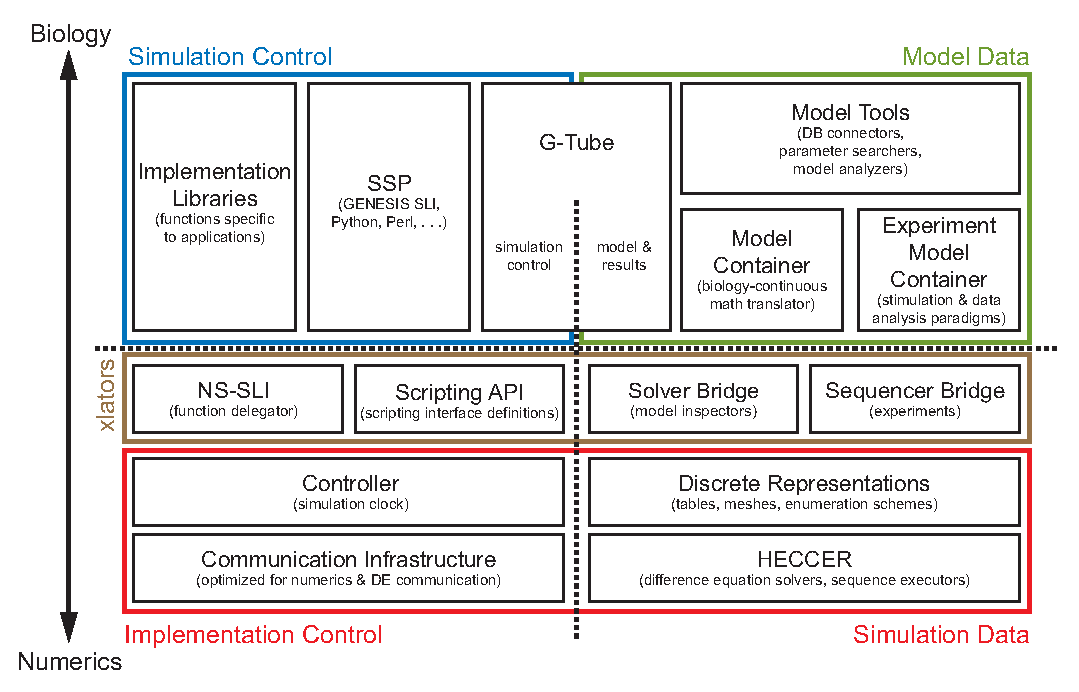
\includegraphics[width=4in]{figures/cbi-g3.eps}
%%  \includegraphics[scale=0.4]{figures/cbi-level2.png}
%\end{center}
%\caption{
%{\bf GENESIS 3.0.}
%The first implementation of the Computational Biology Initiative federated software architecture.
%}
%\label{fig:cbi_g3.eps}
%\end{figure}

%\clearpage


Figure 1

\begin{figure}[ht]
\begin{center}
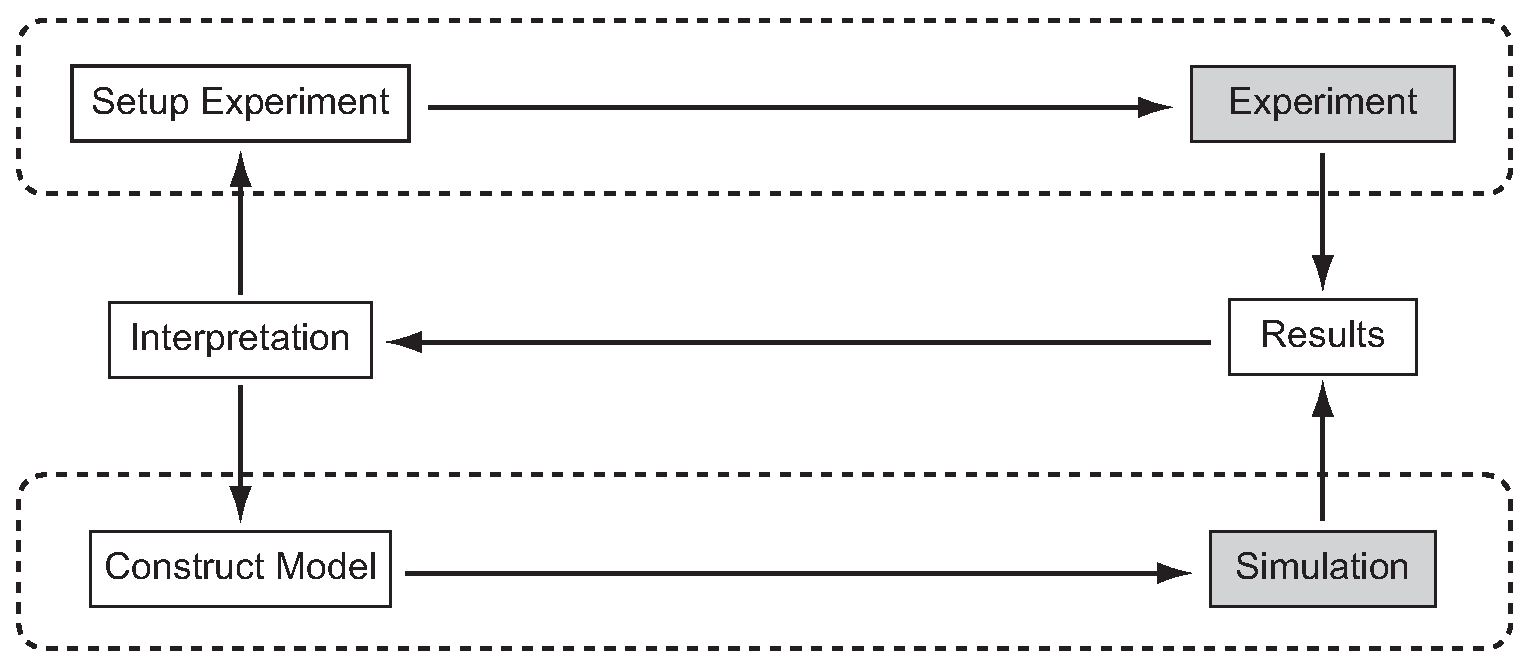
\includegraphics[width=4in]{figures/exp-sim.eps}
\end{center}
\caption{
{\bf Data flows in science.}
Conducting experiments and running simulations are two iterative processes indicated by the upper and lower dashed outlines. They are connected by an interposed feedback loop that uses the iterative interpretation of results to design new experimental setups and model constructions.
}
\label{fig:data-flows}
\end{figure}

\clearpage

Figure 2

\begin{figure}[ht]
\begin{center}
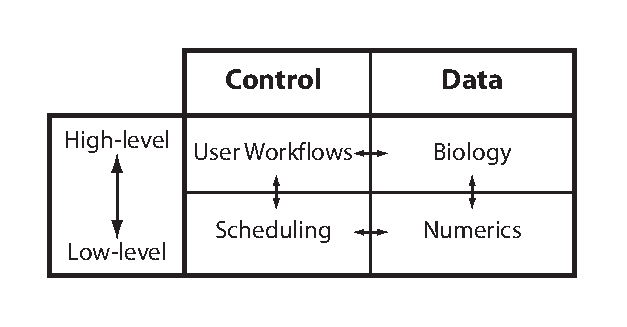
\includegraphics[width=4in]{figures/matrix.eps}
\end{center}
\caption{ {\bf Principle concerns.}  The four fundamental building
  blocks of a simulator are distinguished by separating (i) Data from
  control, and (ii) High level biological concepts from their
  mathematical implementation. In a federated architecture the only
  allowed interactions between modules are those indicated by the
  vertical and horizontal arrows. Diagonal interactions are forbidden
  as they ultimately lead to interactions that result in the existence
  of a monolithic software architecture.
}
\label{fig:data-control}
\end{figure}

\clearpage

Figure 3

\begin{figure}[ht]
\begin{center}
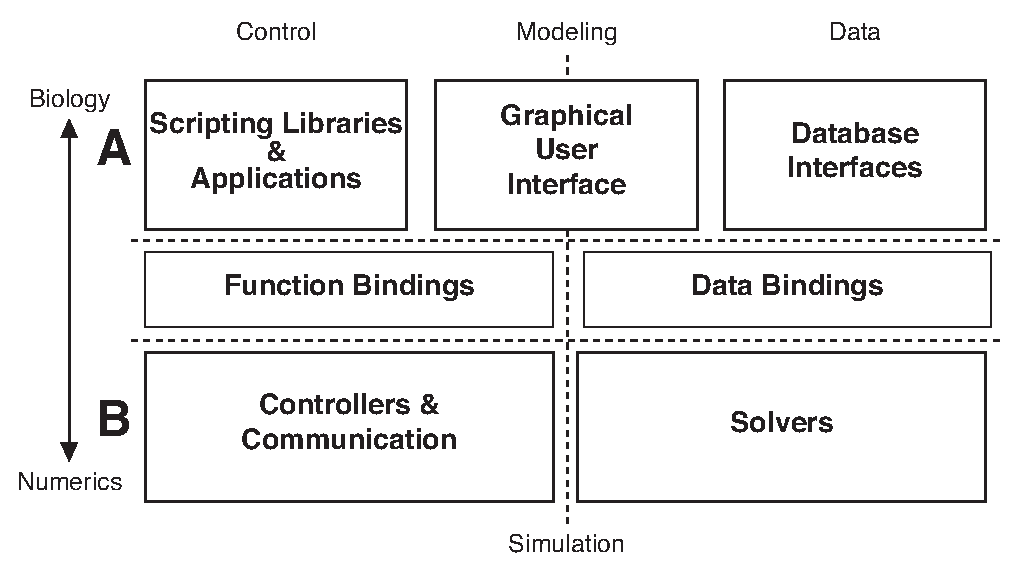
\includegraphics[width=4in]{figures/cbi-architecture-simple.eps}
\end{center}
\caption{ {\bf Overview of a federated software architecture:} Graphical
  illustration of the primary functional modules defined for the CBI
  federated software architecture.  Control modules are given to the left and data modules to the
  right.  A. The top layer contains conceptual data
  and controls representations of the biology of a model. B. The bottom layer contains
  representations that are numeric and thus close to the hardware.  The middle or intermediate layer
  bridges between the biology and the numerics implemented in a CBI compliant simulator. Importantly, as our separation of concerns shows (see Fig. \ref{fig:data-control} and text), Control (Scripting Libraries \& Applications) and Data (Database Interfaces) modules can interact either directly or via the Graphical User Interface.
  }
\label{fig:cbi-architecture-simple}
\end{figure}

\clearpage

Figure 4

\begin{figure}[ht]
\begin{center}
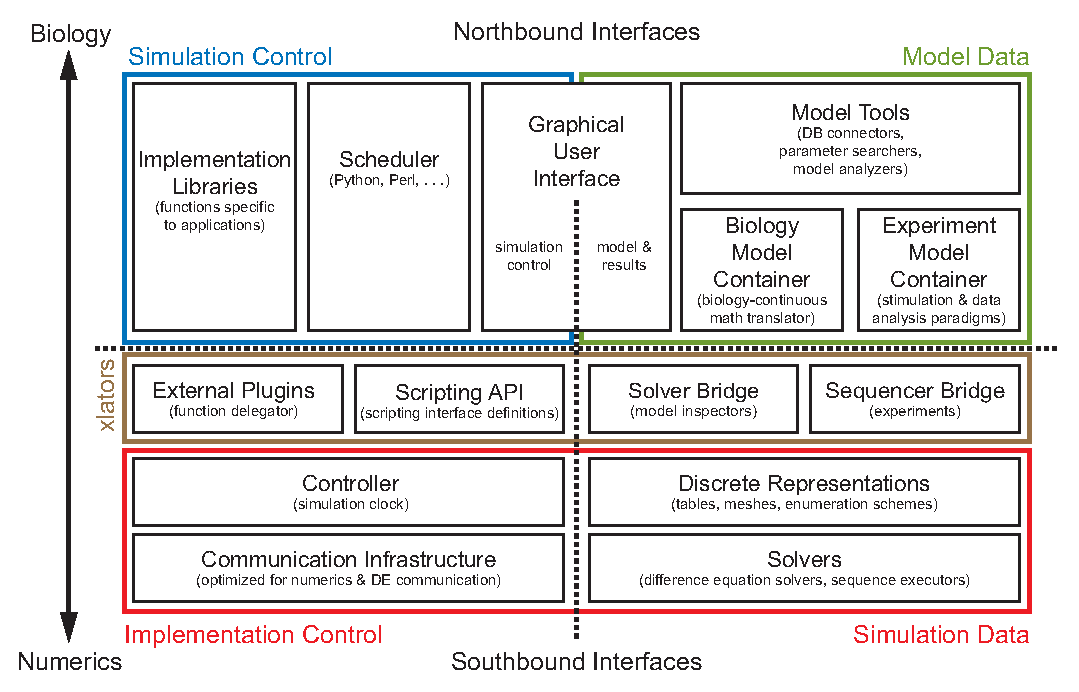
\includegraphics[width=4in]{figures/cbi-architecture-expanded.eps}
\end{center}
\caption{ {\bf Detailed view of the Computational Biology Initiative
    federated software architecture.} Illustration of the functional modules that is closer to an implementation of the CBI architecture. It illustrates the relationships of sub-modules within each of the primary functional modules given in
  Figure \ref{fig:cbi-architecture-simple}.  North bound interfaces
  group and conceptualize the details of the modules and interact with
  south bound interfaces of higher level modules.  Steps 1--3 of the ideal user workflow induce data flows between the software modules of the CBI
architecture. This results in data cycling between the upper layers (blue and green boxes) and
lower layers (red box).  Ultimately, the two layers team to implement a single simulation.  By design, any type of model including multi-scale models will exhibit this data cycle. See text for explanation and details.
}
\label{fig:cbi-architecture-expanded}
\end{figure}

%\section*{Tables}
%\begin{table}[!ht]
%\caption{
%\bf{Table title}}
%\begin{tabular}{|c|c|c|}
%table information
%\end{tabular}
%\begin{flushleft}Table caption
%\end{flushleft}
%\label{tab:label}
% \end{table}

%\begin{table}[!ht]
%\caption{
%\bf{Table title}}
%\begin{tabular}{|c|c|c|}
%%table information
%\end{tabular}
%\begin{flushleft}
%\end{flushleft}
%%\label{tab:cbi-codecounts}
%\end{table}

\end{document}
